% Paquets généraux
\documentclass[a4paper,12pt,titlepage]{article}
\usepackage[T1]{fontenc}
\usepackage[utf8]{inputenc}
\usepackage[french]{babel}
\usepackage[gen]{eurosym}
%\usepackage[dvips]{graphicx}
\usepackage{fancyhdr}
\usepackage{pdfpages} 
\usepackage{multido}
\usepackage{hyperref}
%\usepackage{textcomp}
%\usepackage{aeguill}
\usepackage{schemabloc}
\usepackage[bitstream-charter]{mathdesign}

\newcommand{\id}{54}
\newcommand{\nom}{Liaisons mécaniques}
\newcommand{\sequence}{04}
\newcommand{\num}{01}
\newcommand{\type}{TP}
\newcommand{\descrip}{Modélisation d'un solide. Comportement des liaisons mécaniques. Modéliser les mécanismes du laboratoire par un schéma cinématique, paramétré.}
\newcommand{\competences}{A3-C4: Analyse d'architecture et de comportement \\ &  Mod1-C1: Isolement d'un solide ou d'un système de solides \\ &  Mod2-C10-1: Modèle de solide indéformable \\ &  Mod2-C11: Modélisation géométrique et cinématique des mouvements entre solides indéformables \\ &  Mod2-C12: Modélisation cinématique des liaisons entre solides \\ &  Mod2-C15: Modélisation des actions mécaniques \\ &  Rés-C6: Utilisation d'un solveur ou d'un logiciel multi physique \\ &  Com1-C1: Différents descripteurs introduits dans le programme \\ &  Com2-C4: Outils de communication}
\newcommand{\nbcomp}{9}
\newcommand{\systemes}{Plateforme Stewart}
\newcommand{\systemessansaccent}{Plateforme Stewart}
\newcommand{\ilot}{2}
\newcommand{\ilotstr}{02}
\newcommand{\dossierilot}{\detokenize{Ilot_02 Plateforme Stewart}}
\newcommand{\imageun}{Plateforme}

\newcommand{\urlsysteme}{\href{https://www.costadoat.fr/systeme/57}{Ressources système}}
\newcommand{\matlabsimscape}{\href{https://github.com/Costadoat/Sciences-Ingenieur/raw/master/Systemes/Plateforme Stewart/Plateforme_Stewart_Simscape.zip}{Modèle Simscape}}
\newcommand{\solidworks}{\href{https://github.com/Costadoat/Sciences-Ingenieur/raw/master/Systemes/Plateforme Stewart/Plateforme_Stewart_Solidworks.zip}{Modèle Solidworks}}
\newcommand{\edrawings}{\href{https://github.com/Costadoat/Sciences-Ingenieur/raw/master/Systemes/Plateforme Stewart/Plateforme_Stewart.EASM}{Modèle eDrawings}}
\newcommand{\test}{Stewart_param1}
\newcommand{\testi}{Stewart_param2}
\newcommand{\testii}{Stewart_param3}
\newcommand{\testiii}{Stewart_param4}
\newcommand{\testiiii}{Stewart_euler}

\newcommand{\auteurun}{Renaud Costadoat}
\newcommand{\auteurdeux}{Françoise Puig}
\newcommand{\institute}{Lycée Dorian}


\usepackage{color}
\usepackage{xcolor}
\usepackage{colortbl}
\usepackage{helvet}
\renewcommand{\familydefault}{\sfdefault}
\usepackage{amsfonts}
\usepackage{amsmath}
%\usepackage{xspace}
\usepackage{varioref}
\usepackage{tabularx}
%\usepackage{floatflt}
\usepackage{graphics}
\usepackage{wrapfig}
\usepackage{textcomp}
\usepackage{tikz}
\usepackage{wrapfig}
\usepackage{gensymb}
\usepackage[european]{circuitikz}
\usetikzlibrary{babel}
\usepackage{ifthen}
\usepackage{cancel}
\usepackage{etoolbox}
\usepackage{multirow}
%\usepackage{boxedminipage}
\definecolor{gris25}{gray}{0.75}
\definecolor{bleu}{RGB}{18,33,98}
\definecolor{bleuf}{RGB}{42,94,171}
\definecolor{bleuc}{RGB}{231,239,247}
\definecolor{rougef}{RGB}{185,18,27}
\definecolor{rougec}{RGB}{255,188,204}%255,230,231
\definecolor{vertf}{RGB}{103,126,82}
\definecolor{vertc}{RGB}{220,255,191}
\definecolor{forestgreen}{rgb}{0.13,0.54,0.13}
\definecolor{blcr}{rgb}{0.59,0.69,0.84}
\definecolor{blfr}{rgb}{0.32,0.51,0.75}
\definecolor{orfr}{rgb}{0.90,0.42,0.15}
\definecolor{orcr}{rgb}{0.90,0.65,0.50}
\definecolor{orangef}{rgb}{0.659,0.269,0.072}
\definecolor{orange}{rgb}{0.58,0.35,0.063}
\definecolor{orangec}{rgb}{0.43,0.32,0.25}
\definecolor{rcorrect}{rgb}{0.6,0,0}
\definecolor{sequence}{rgb}{0.75,0.75,0.75}
\definecolor{competences}{rgb}{0.61,0.73,0.35}
\definecolor{grisf}{HTML}{222222}
\definecolor{grisc}{HTML}{636363}
\definecolor{normal}{HTML}{4087c4}
\definecolor{info}{HTML}{5bc0de}
\definecolor{success}{RGB}{92,184,92}
\definecolor{warning}{RGB}{240,173,78}
\definecolor{danger}{RGB}{217,83,79}
\hypersetup{                    % parametrage des hyperliens
    colorlinks=true,                % colorise les liens
    breaklinks=true,                % permet les retours à la ligne pour les liens trop longs
    urlcolor= blfr,                 % couleur des hyperliens
    linkcolor= orange,                % couleur des liens internes aux documents (index, figures, tableaux, equations,...)
    citecolor= forestgreen                % couleur des liens vers les references bibliographiques
    }

% Mise en page
\pagestyle{fancy}

\setlength{\hoffset}{-18pt}

\setlength{\oddsidemargin}{0pt} 	% Marge gauche sur pages impaires
\setlength{\evensidemargin}{0pt} 	% Marge gauche sur pages paires
\setlength{\marginparwidth}{00pt} 	% Largeur de note dans la marge
\setlength{\headwidth}{481pt} 	 	% Largeur de la zone de tête (17cm)
\setlength{\textwidth}{481pt} 	 	% Largeur de la zone de texte (17cm)
\setlength{\voffset}{-18pt} 		% Bon pour DOS
\setlength{\marginparsep}{7pt}	 	% Séparation de la marge
\setlength{\topmargin}{-30pt} 		% Pas de marge en haut
\setlength{\headheight}{35pt} 		% Haut de page
\setlength{\headsep}{20pt} 		% Entre le haut de page et le texte
\setlength{\footskip}{30pt} 		% Bas de page + séparation
\setlength{\textheight}{700pt} 		% Hauteur de l'icone zone de texte (25cm)
\setlength\fboxrule{1 pt}
\renewcommand{\baselinestretch}{1}
\setcounter{tocdepth}{1}
\newcommand{\cadre}[2]
{\fbox{
  \begin{minipage}{#1\linewidth}
   \begin{center}
    #2\\
   \end{center}
  \end{minipage}
 }
}

\newcounter{num_quest} \setcounter{num_quest}{0}
\newcounter{num_rep} \setcounter{num_rep}{0}
\newcounter{num_cor} \setcounter{num_cor}{0}

\newcommand{\question}[1]{\refstepcounter{num_quest}\par
~\ \\ \parbox[t][][t]{0.15\linewidth}{\textbf{Question \arabic{num_quest}}}\parbox[t][][t]{0.93\linewidth}{#1}\par
}


\newcommand{\reponse}[1]
{\refstepcounter{num_rep}
\noindent
\rule{\linewidth}{.5pt}
\textbf{Question \arabic{num_rep}:}
\multido{\i=1+1}{#1}{~\ \\}
}

\newcommand{\cor}
{\refstepcounter{num_cor}
\noindent
\rule{\linewidth}{.5pt}
\textbf{Question \arabic{num_cor}:} \\
}

\newcommand{\titre}[1]
{\begin{center}
\cadre{0.8}{\huge #1} 
\end{center}
}


% En tête et pied de page
\fancypagestyle{normal}{%
  \fancyhf{}
\lhead{\nom}
\rhead{
\includegraphics[width=2cm]{../../img/logo}\hspace{2pt}}
\ifdef{\auteurdeux}{\lfoot{\auteurun,\auteurdeux}}{\lfoot{\auteurun}}
\cfoot{Page \thepage}}

\fancypagestyle{correction}{%
  \fancyhf{}
  \lhead{\colorbox{danger}{\begin{minipage}{0.65\paperwidth} \textcolor{white}{\textbf{Correction}} \end{minipage}} }
  \rhead{
\includegraphics[width=2cm]{../../img/logo}}
  \ifdef{\auteurdeux}{\lfoot{\auteurun,\auteurdeux}}{\lfoot{\auteurun}}
  \rfoot{\colorbox{danger}{\begin{minipage}{0.5\paperwidth} \begin{flushright}\textcolor{white}{\textbf{Correction}}\end{flushright} \end{minipage}} }}

\renewcommand{\footrulewidth}{0.4pt}

\usepackage{eso-pic}
\newcommand{\BackgroundPic}{%
\put(0,0){%
\parbox[b][\paperheight]{\paperwidth}{%
\vfill
\begin{center}
\hspace{0.5cm}\vspace{0.5cm}

\includegraphics[width=\paperwidth,height=\paperheight,%
keepaspectratio]{../../img/fond3}%
\end{center}
\vfill
}}}

\newcommand{\BackgroundPicdeux}{%
\put(25,-30){%
\parbox[b][\paperheight]{\paperwidth}{%
\vfill
\begin{center}
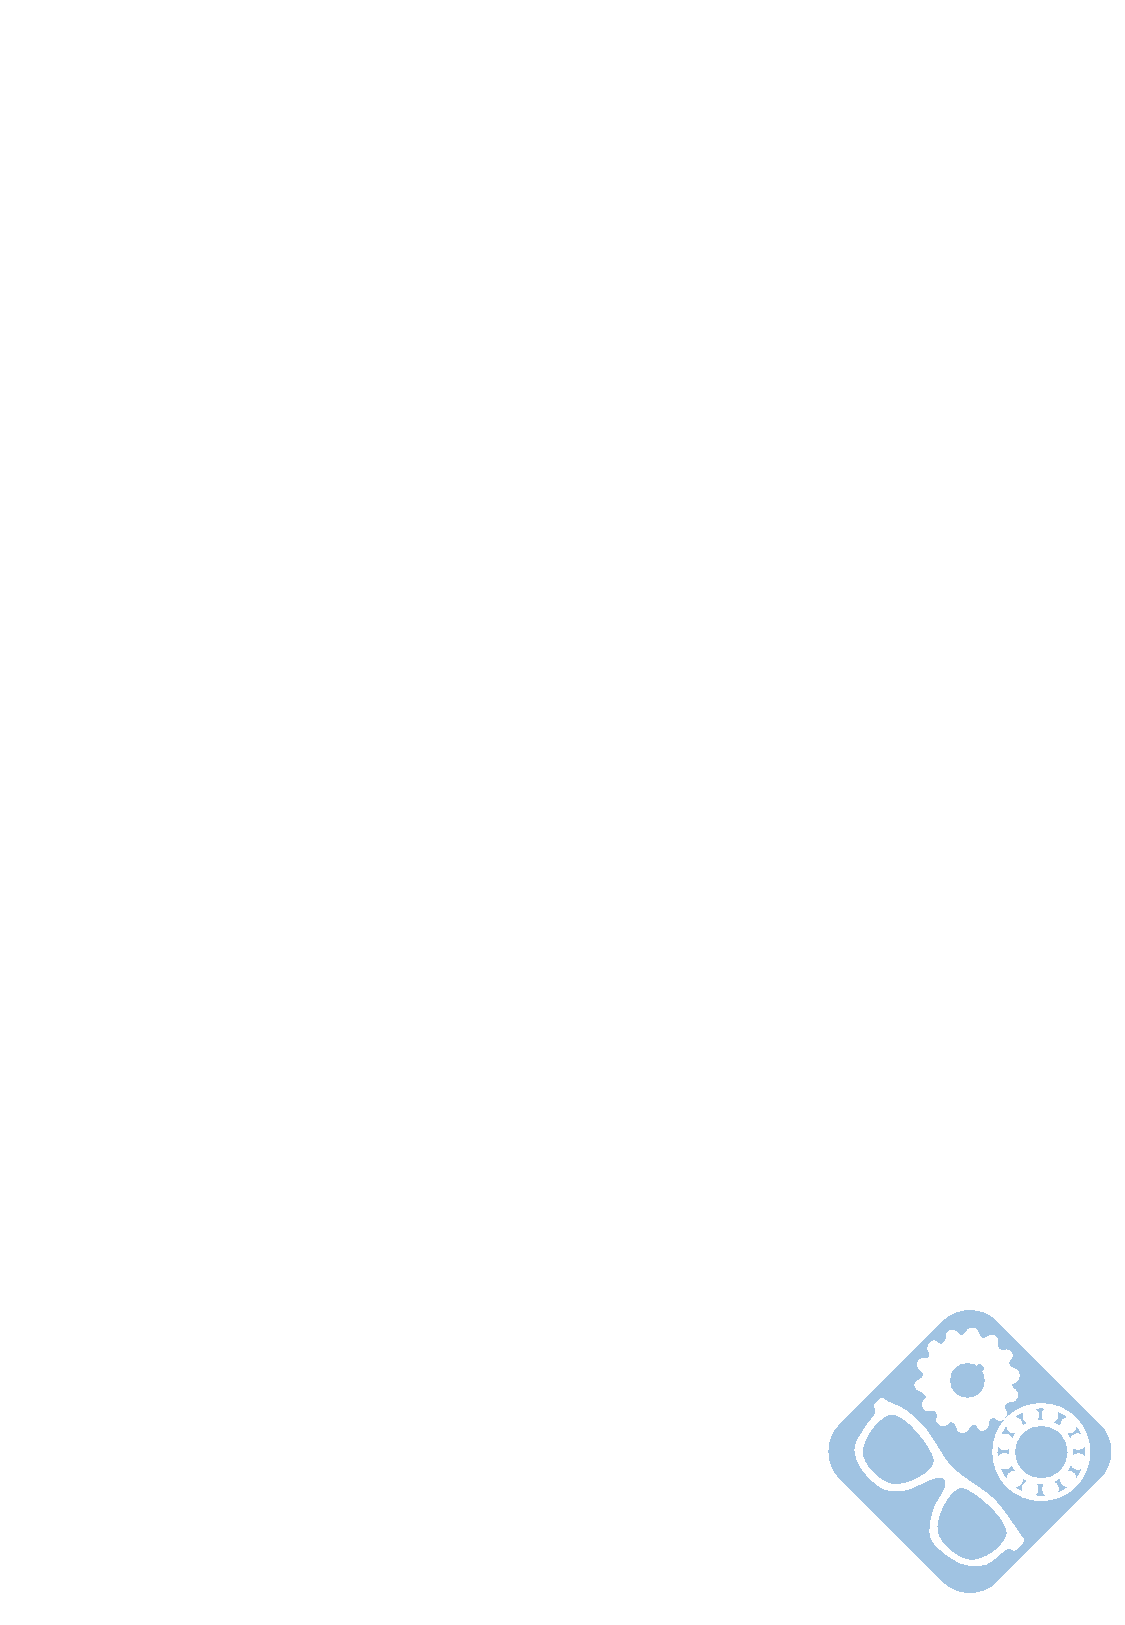
\includegraphics[width=\paperwidth,height=\paperheight,%
keepaspectratio]{../../img/fond4}%
\end{center}
\vfill
}}}

\begin{document}

\pagestyle{empty}

\vspace*{-3\baselineskip}

\AddToShipoutPicture*{\BackgroundPic}

\ifdef{\auteurdeux}{\begin{tabular}{>{\columncolor{gray!00}}m{.3\linewidth} m{.3\linewidth} >{\columncolor{gray!00}}m{.3\linewidth}}
Séquence : \sequence &  \multirow{3}{*}{\hspace{1cm}
\includegraphics[height=1.5cm]{../../img/logo}} &  \begin{flushright} \multirow{4}{*}{\hspace{1cm}
\includegraphics[height=4cm]{img/qrcode}}\end{flushright}\\
Document : \type\num \\
 \institute \\
 \auteurun\\
 \auteurdeux
\end{tabular}}{\begin{tabular}{>{\columncolor{gray!00}}m{.3\linewidth} m{.3\linewidth} >{\columncolor{gray!00}}m{.3\linewidth}}
Séquence : \sequence &  \multirow{3}{*}{\hspace{1cm}
\includegraphics[height=1.5cm]{../../img/logo}} &  \begin{flushright} \multirow{4}{*}{\hspace{1cm}
\includegraphics[height=4cm]{img/qrcode}}\end{flushright}\\
Document : \type\num \\
 \institute \\
 \auteurun
\end{tabular}}

\vspace{1cm}

\ifdef{\prive}{\begin{center}\colorbox{danger}{\Huge{Avec Correction}}\end{center}}{}

\begin{center}\huge{\nom}\end{center}

\vspace{2cm}

\ifdef{\imagedeux}{\begin{minipage}{0.49\linewidth}}{}
\begin{center}\includegraphics[height=5cm]{/home/renaud/Documents/Renaud/GitHub/django_education/systemes/\imageun}\end{center}
\ifdef{\imagedeux}{\end{minipage}\hfill
\begin{minipage}{0.49\linewidth}
\begin{center}\includegraphics[height=5cm]{/home/renaud/Documents/Renaud/GitHub/django_education/systemes/\imagedeux}\end{center}
\end{minipage}}{}

\vspace{5cm}


\begin{tabular}{p{.15\linewidth} >{\columncolor{white}}p{.8\linewidth}}
    \rowcolor{gray!20}
    Référence & S\sequence\ - \type\num \\
    Compétences & \competences \\
 	\rowcolor{gray!20}
    Description & \descrip \\
    Système & \systemes
  \end{tabular}

\newpage

\AddToShipoutPicture{\BackgroundPicdeux}

\pagestyle{normal}

\section{Motorisation d'un axe vertical de plateau tournant}

Le plateau-tournant (3), représenté ci-dessous, est en rotation par rapport au carter principal (1) selon un axe vertical $(O',\overrightarrow{z'_1})$. Un réducteur de rapport de réduction $r=\frac{\omega_3}{\omega_2}$ est placé entre l'arbre de sortie de moteur (2) et l'arbre lié au plateau (3). L'arbre de sortie de moteur (2), équipé d'un pignon en bout, a un moment d'inertie $J_2$ par rapport à l'axe $(O,\overrightarrow{z_1})$. L'arbre lié au plateau (3), équipé d'un pignon en bout, a un moment d'inertie $J_3$ par rapport à l'axe $(O',\overrightarrow{z'_1})$.

\begin{figure}[!h]
 \centering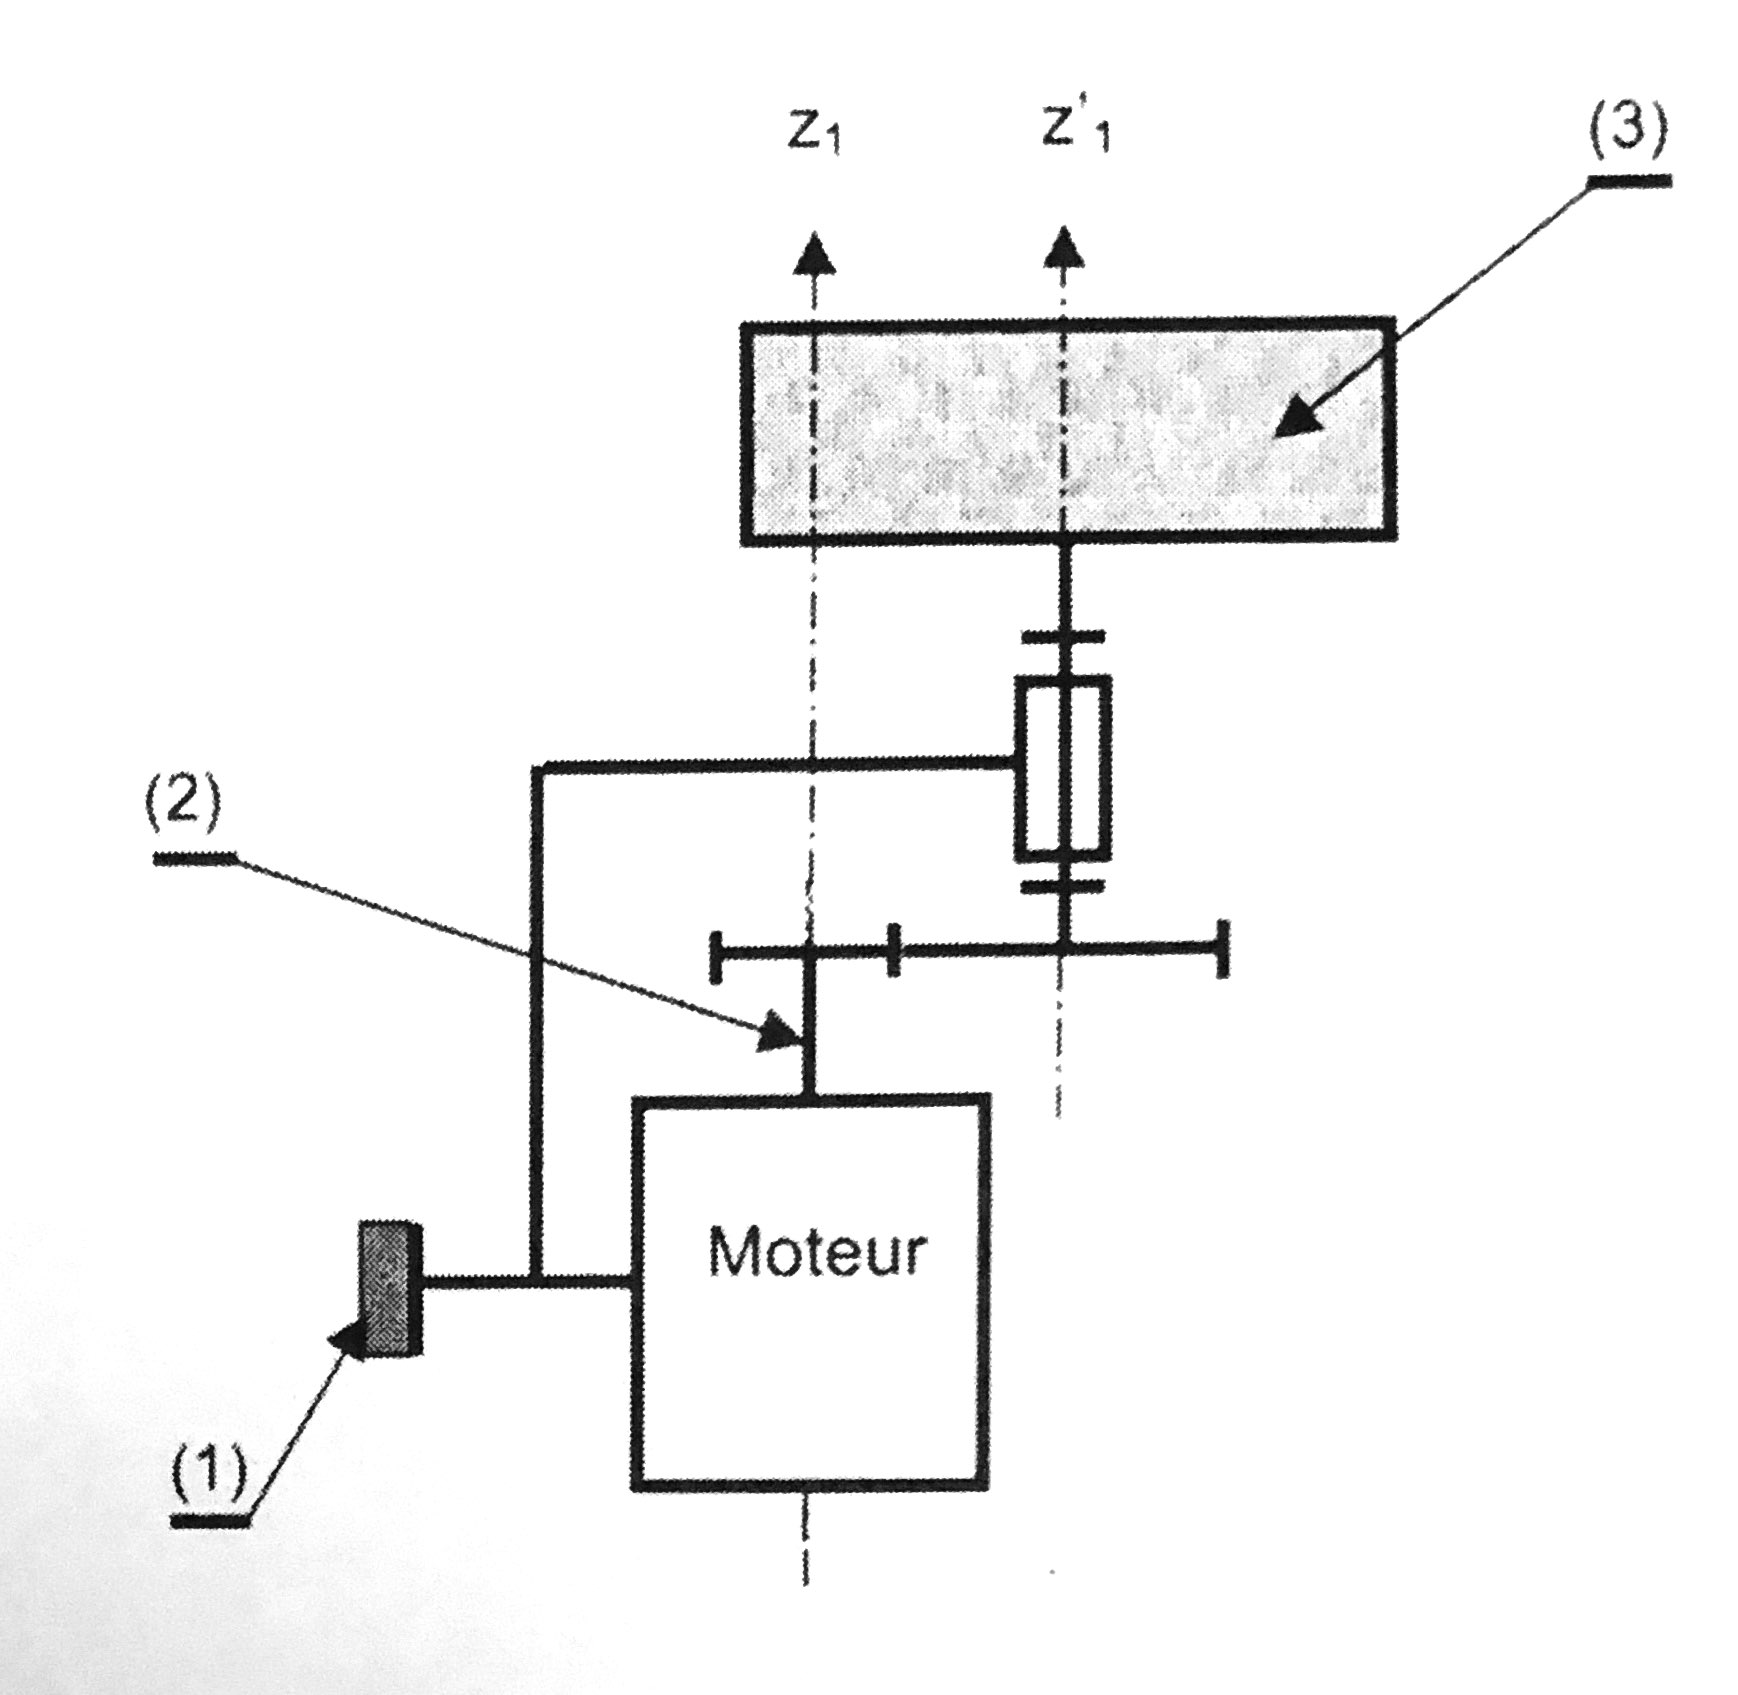
\includegraphics[width=0.6\linewidth]{img/fig_moteur_charge_01}
  \caption{Motorisation d'un axe vertical}
 \label{fig_moteur_charge_01}
\end{figure}

Les équations du moteur à courant continu sont les suivantes:
\begin{eqnarray}
u(t)=R.i(t)+e(t) \\
e(t)=K_e.\omega_2(t) \\
C_m(t)=K_c.i(t) \\
C_m(t)=J_i.\frac{d\omega_2(t)}{dt}
\end{eqnarray}

Avec:
\begin{itemize}
 \item $u(t)$ (en $V$), tension de l'induit,
 \item $R=1,1\ \Omega$, résistance de l'induit,
 \item $i(t)$ (en $A$), intensité du courant d'induit,
 \item $e(t)$ (en $V$), force électromotrice (on néglige l'inductance de l'induit L ),
 \item $\omega_2(t)$ (en $rad.s^{-1}$) vitesse de rotation de l'arbre de sortie de moteur (2),
 \item $K_e=0,265\ V.rad^{-1}.s$ constante électrique du moteur
 \item $C_m(t)$ (en $N.m$), couple moteur,
 \item $K_c=0,025\ N.m.A^{-1}$ constante de couple,
 \item $J_i$ (en $kg.m^2$), moment d'inertie ramené sur l'arbre de sortie de moteur (2).
\end{itemize}

\subsection{Moteur seul}

Pour cette partie, on prendra $J_i=J_2$ pour l'équation (4).

\paragraph{Question 1:} Écrire les équations du moteur dans le domaine de Laplace (les conditions initiales sont nulles), et citer le(s) théorème(s) utilisé(s).

\paragraph{Question 2:} Trouver une relation entre $U(p)$ et $\Omega_2(p)$.

\paragraph{Question 3:} Mettre la relation précédente sous la forme
$H(p)=\frac{\Omega_2(p)}{U(p)}=\frac{K_m}{1+\tau_m.p}$. Préciser les expressions littérale de $K_m$ et $\tau_m$.

Une génératrice tachymétrique, placée sur l'arbre de sortie du moteur (2), relève sa vitesse de rotation.

Une tension d'entrée en échelon $u(t)=u_0=25\ V$ produit la courbe $\omega_2(t)=f(t)$ suivante:

\begin{figure}[!h]
 \centering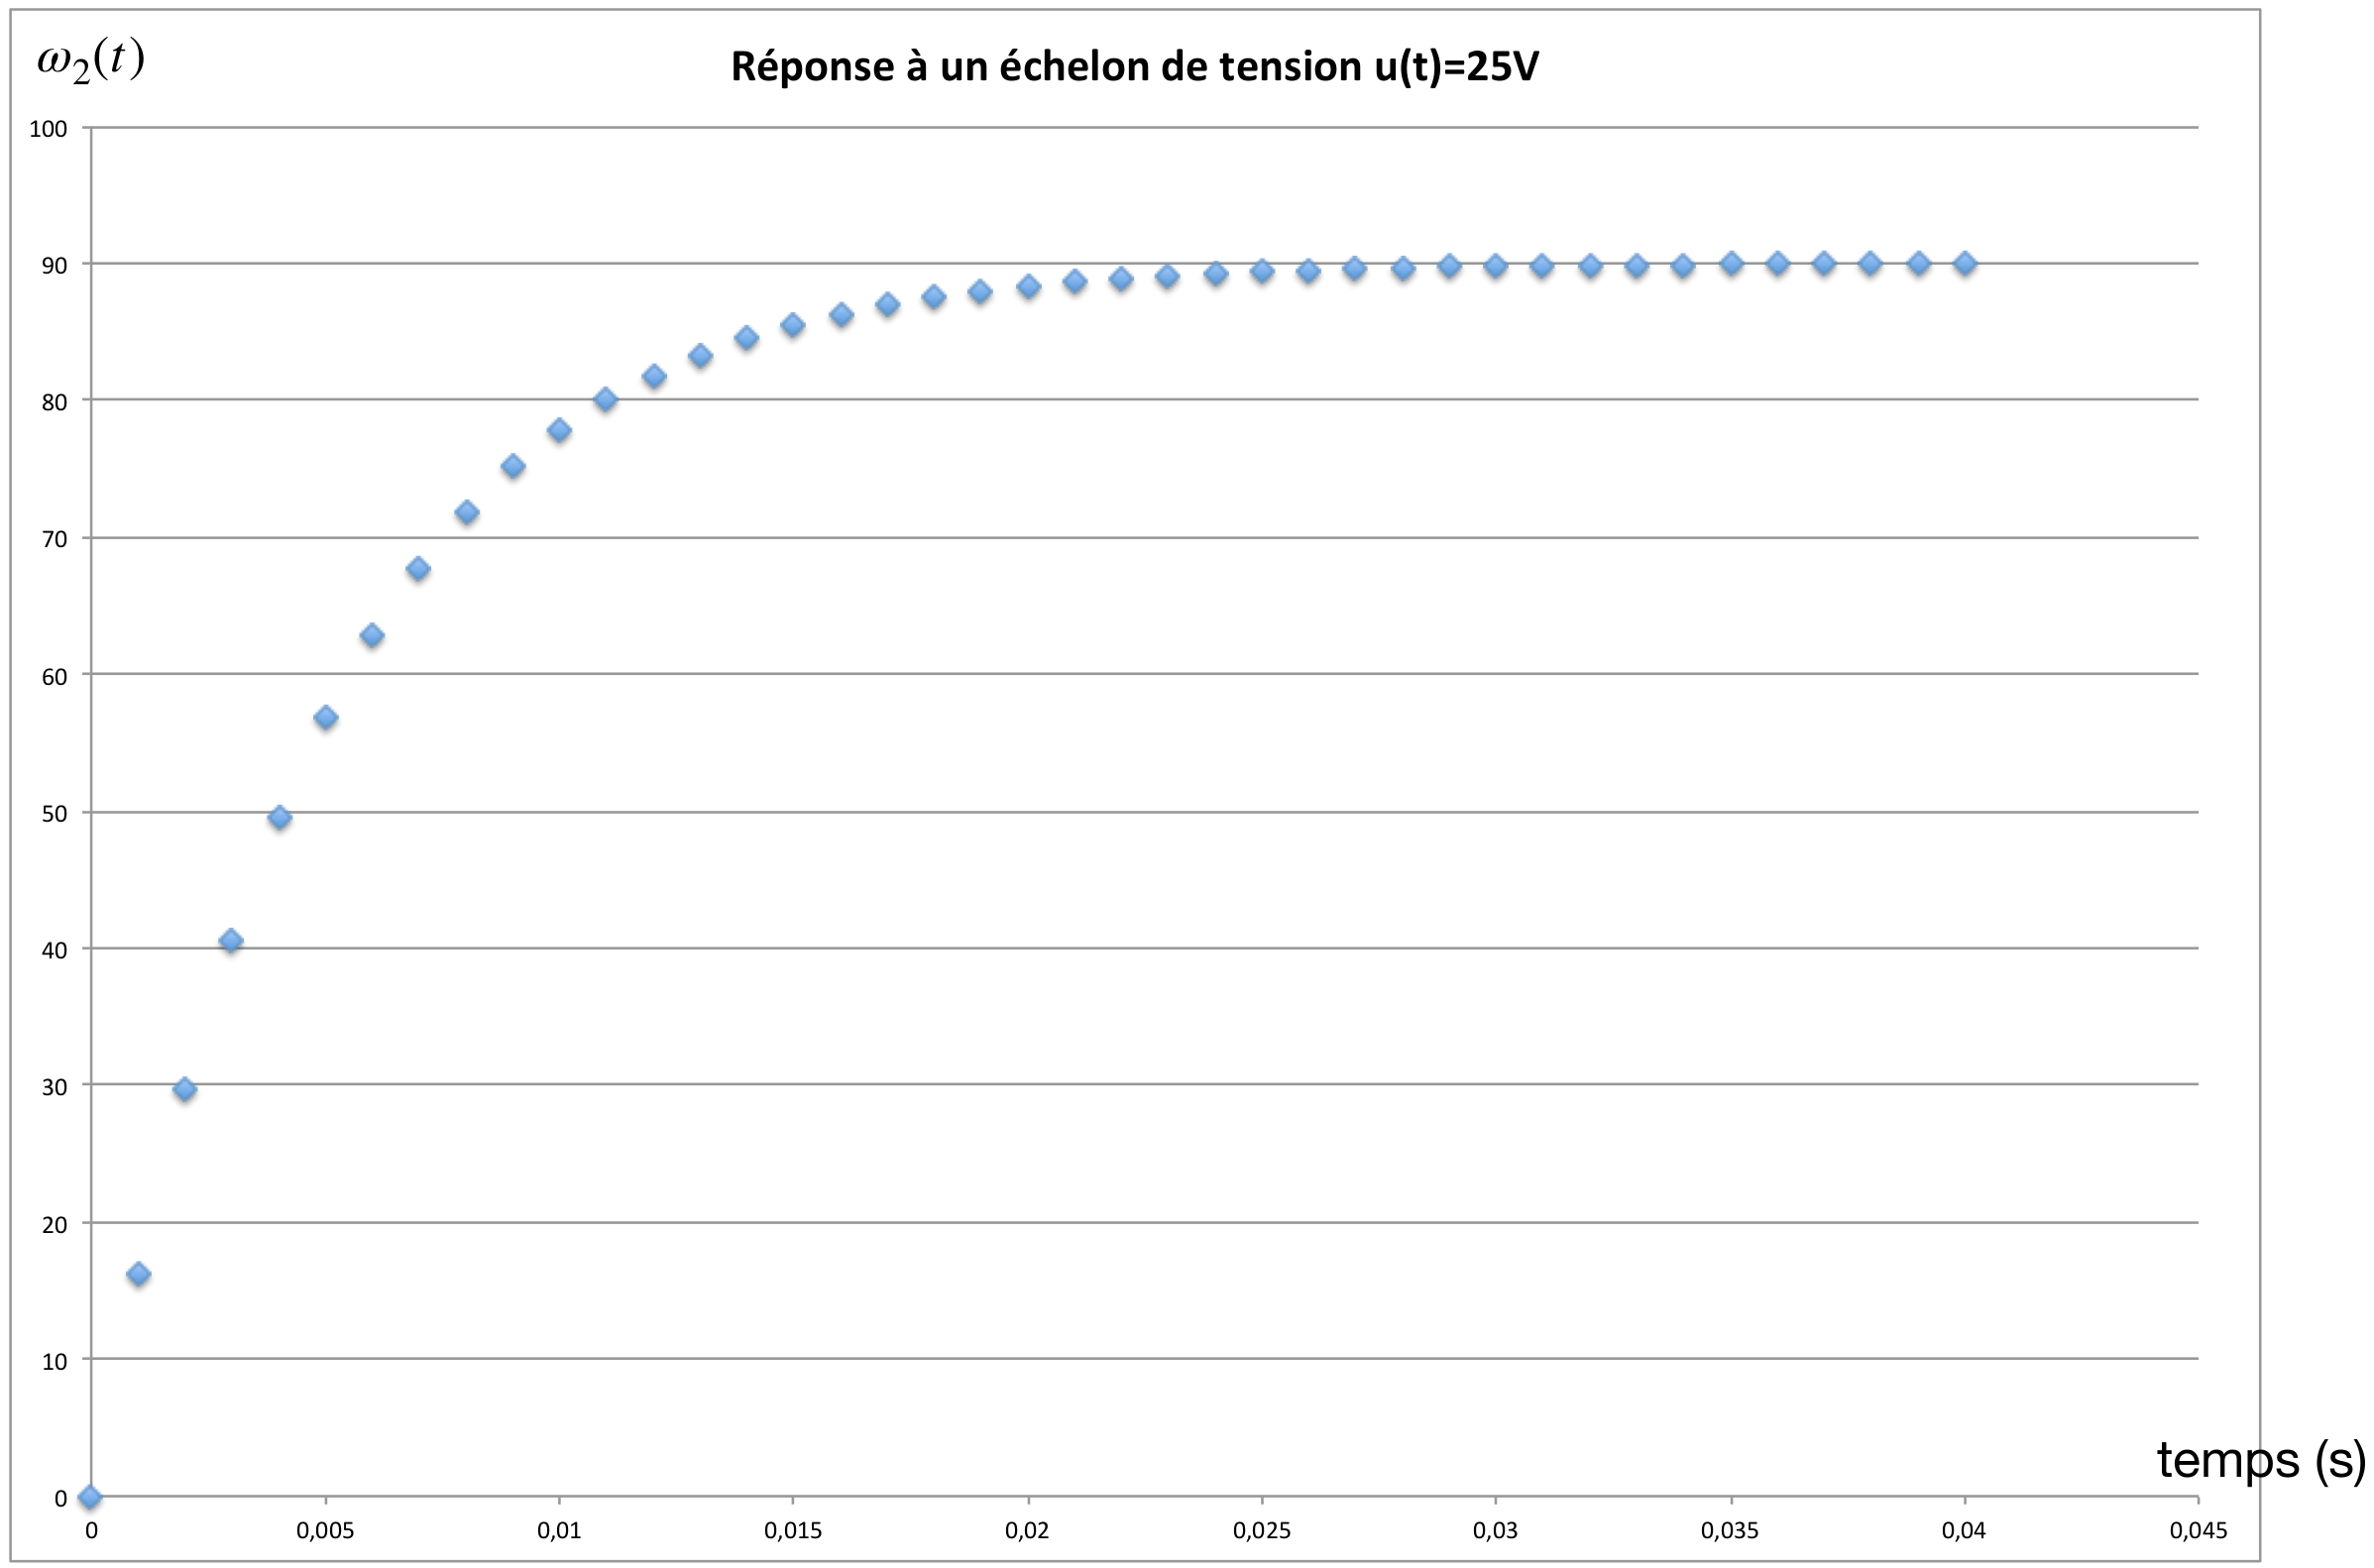
\includegraphics[width=0.8\linewidth]{img/fig_moteur_charge_02}
  \caption{Mesure génératrice tachymétrique}
 \label{fig_moteur_charge_02}
\end{figure}

\paragraph{Question 4:} Déterminer les valeurs numériques des constantes $K_m$ et $\tau_m$.

\paragraph{Question 5:} En déduire le moment d'inertie $J_2$ de l'arbre de sortie du moteur (2).

\newpage

\subsection{Moteur en charge}

En utilisant le théorème de l'énergie cinétique, on montre que le moment d'inertie de l'ensemble \{moteur+charge\}, ramené sur l'arbre de sortie du moteur (2) a pour expression:

$J_i=J_T=J_2+r_2.J_3$ avec $r=\frac{\omega_3}{\omega_2}=\frac{1}{50}$

\paragraph{Question 6:} Écrire la nouvelle fonction de transfert
$H_T(p)=\frac{\Omega_2(p)}{U(p)}$ et la mettre sous forme canonique
$H_T(p)=\frac{\Omega_2(p)}{U(p)}=\frac{K_T}{1+\tau_T.p}$. Préciser les expressions littérale de $K_T$ et $\tau_T$.

\paragraph{Question 7:} Écrire le rapport entre $\tau_T$ et $\tau_m$.

La génératrice tachymétrique, placée sur l'arbre de sortie du moteur (2), relève sa vitesse de rotation.

Une tension d'entrée en échelon $u(t)=u_0=25\ V$ produit la courbe $\omega_2(t)=f(t)$ suivante:

\begin{figure}[!h]
 \centering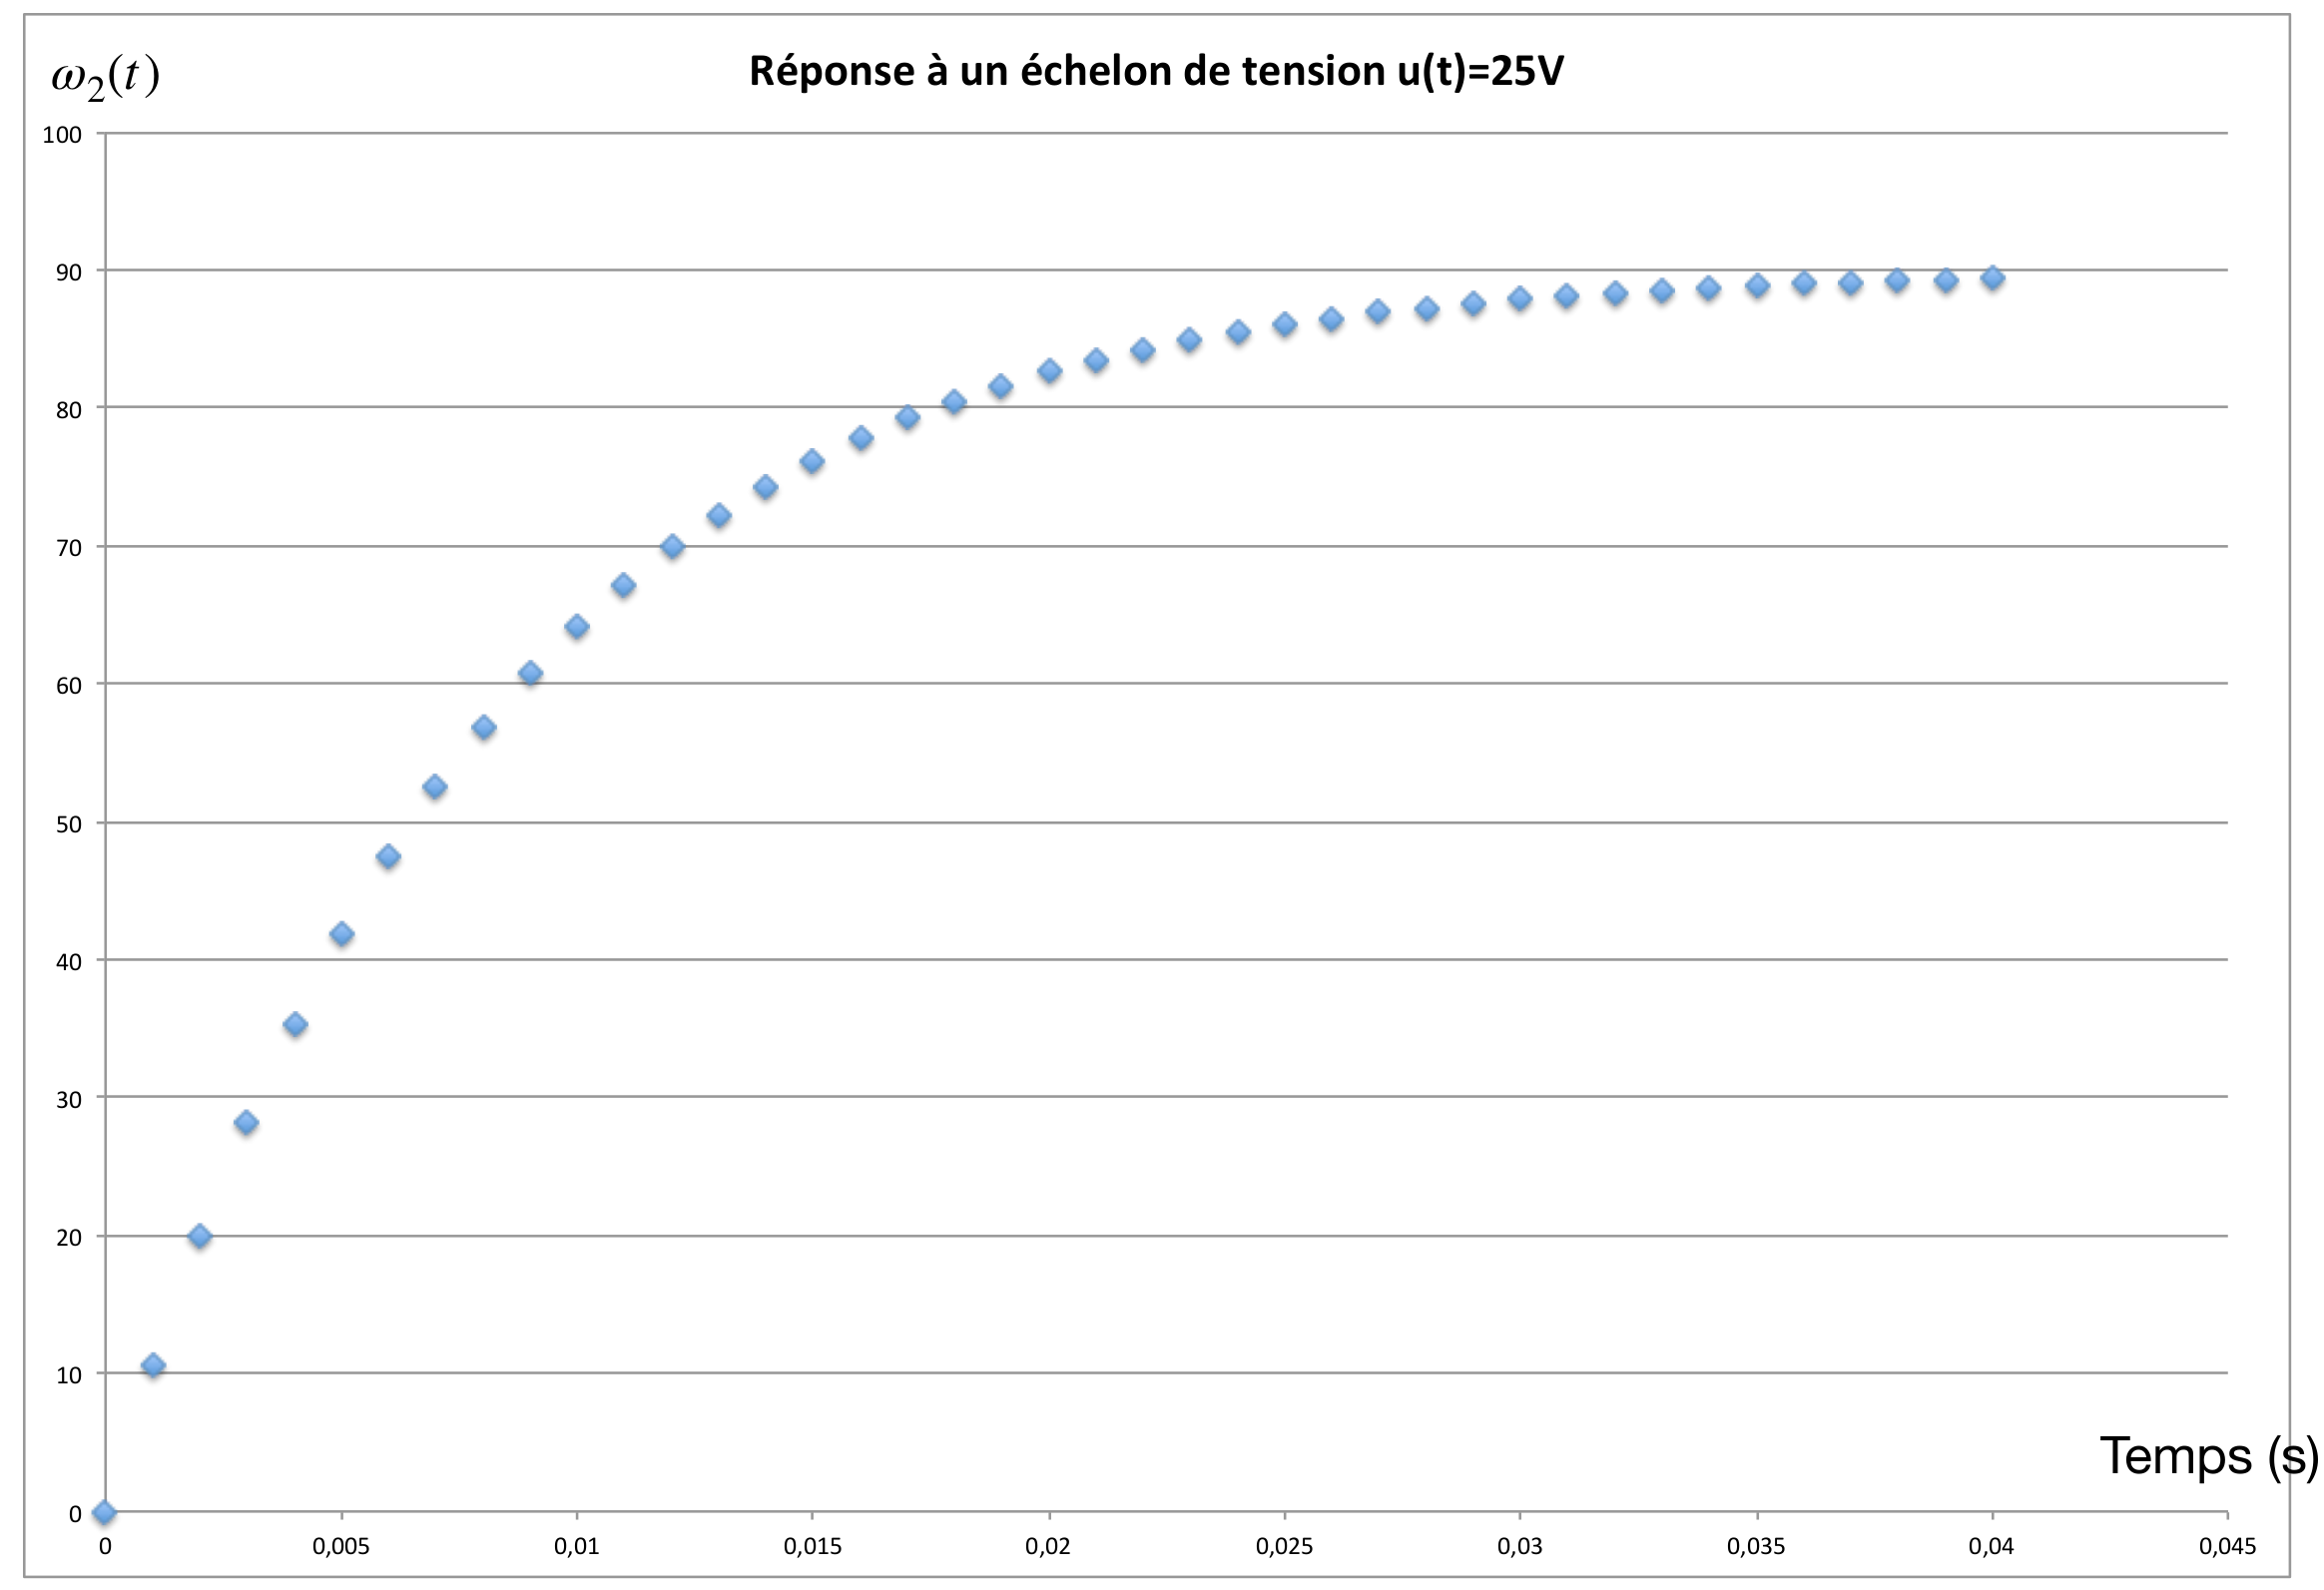
\includegraphics[width=0.8\linewidth]{img/fig_moteur_charge_03}
  \caption{Mesure génératrice tachymétrique 2}
 \label{fig_moteur_charge_03}
\end{figure}

\newpage

\section{Maxpid}

\subsection{Description du moteur à courant continu}

\begin{minipage}{0.6\linewidth}
L'actionneur moteur est un moteur électrique à courant continu MAXON RE035G utilisé sur la chaîne cinématique asservie du système didactique MAXPID de la société PELENC. Ce type d'architecture équipe des robots cueilleurs de fruit produits par cette même société.
\end{minipage}
 \hfill
\begin{minipage}{0.35\linewidth}
 \centering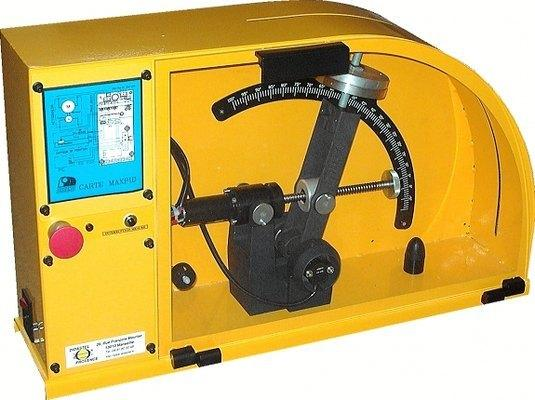
\includegraphics[width=0.8\linewidth]{img/Maxpid.png}
\end{minipage}

Caractéristiques du moteur:
\begin{center}
\begin{tabular}{|c|c|c|}
\hline
Tension d'alimentation $(U_a)$ & $V$ & 24 \\
\hline
Vitesse au courant $I_n$ & $tr.min^{-1}$ & 3493 \\
\hline
Couple au courant $I_n$ & $mN.m$ & 113 \\
\hline
Courant max permanent $(I_n)$ & $mA$ & 2150 \\
\hline
Vitesse à vide à $U_a$ $\pm 10\%$ & $tr.min^{-1}$ & 4303 \\
\hline
Courant à vide à $\pm 50\%$ & $mA$ & 92.8 \\
\hline
Couple de démarrage à $U_a$ & $mN.m$ & 611\\
\hline
Courant de démarrage à $U_a$ & $mA$ &  11600 \\
\hline
Constante de couple & $mN.m.A^{-1}$ & 52.5 \\
\hline
Constante de vitesse & $tr.min^{-1}.V^{-1}$ & 182 \\
\hline
Pente vitesse/couple & $tr.min^{-1}.mN^{-1}.m^{-1}$ & 7.17 \\
\hline
Vitesse limite & $tr.min^{-1}$ & 8200 \\
\hline
Puissance utile max à $U_a$ & $W$ & 69 \\
\hline
Rendement maximum & \% & 85.5 \\
\hline
Constante de temps électromécanique & $ms$ & 5.23 \\
\hline
Inertie & $g.cm^2$ & 69.6 \\
\hline
Résistance aux bornes & $Ohm$ & 2.07 \\
\hline
Inductivité & $mH$ & 0.62 \\
\hline
Résistance thermique Boîtier/Ambiant & $K.W^{-1}$ & 6.2 \\
\hline
Résistance thermique Rotor/Boîtier & $K.W^{-1}$ & 2 \\
\hline
\end{tabular}
\end{center}

\subsection{Modélisation du servomoteur à courant continu}

Le moteur électrique à courant est constitué (voir figure \ref{maxpid1}) :
\begin{itemize}
 \item d'un rotor appelé induit (bobinage parcouru par un courant i),
 \item d'un stator appelé inducteur,
 \item d'un ensemble de balais porte-balais pour pouvoir alimenter le rotor en tension lors
de la rotation.
\end{itemize}

\begin{figure}[!h]
 \centering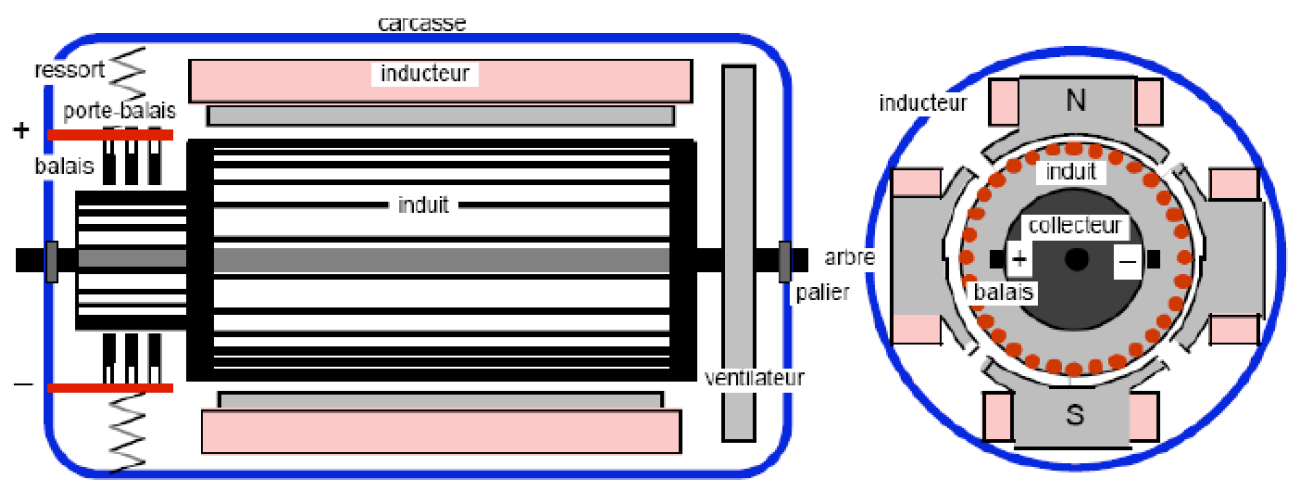
\includegraphics[width=0.65\linewidth]{img/maxpid1.png}
 \caption{Moteur électrique}
 \label{maxpid1}
\end{figure}

Le schéma de principe du moteur à courant continu est donné à la figure suivante :

\begin{figure}[!h]
 \centering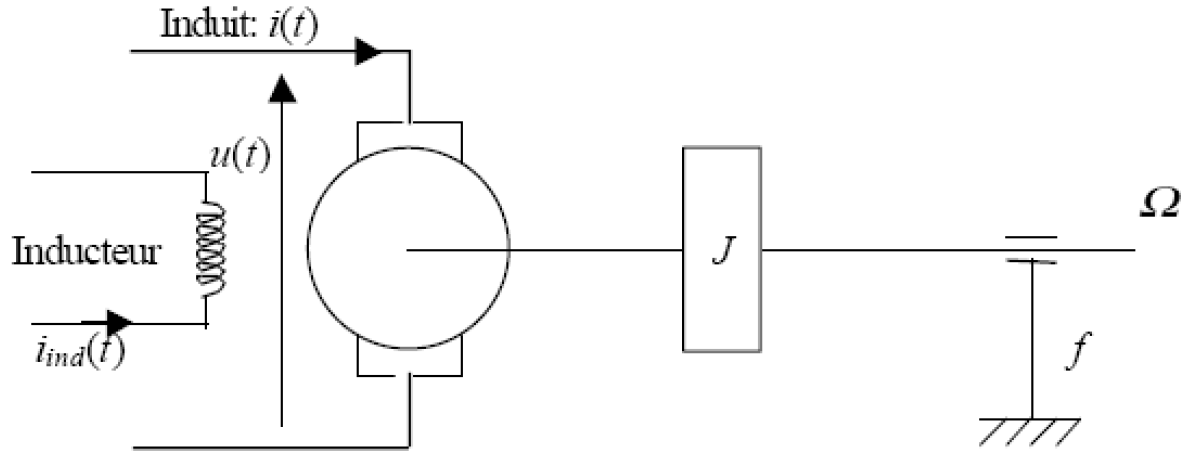
\includegraphics[width=0.7\linewidth]{img/maxpid2.png}
 \caption{Schéma du moteur}
 \label{maxpid2}
\end{figure}

Les bobines de l'inducteur sont alimentées par une intensité $i_{ind}$ électrique constante. Elles produisent un champ magnétique constant qui agit sur l'induit.

L'induit du moteur est alimenté par une tension $u(t)$.

\begin{figure}[!h]
\begin{minipage}{0.45\linewidth}
 \centering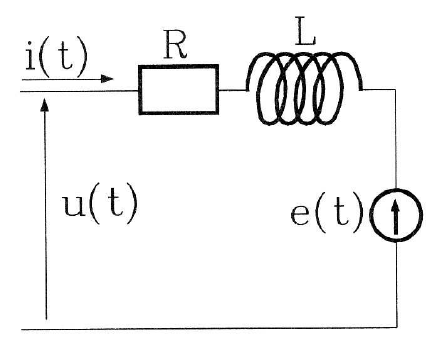
\includegraphics[width=0.7\linewidth]{img/maxpid3.png}
  \caption{Schéma électrique}
 \label{maxpid3}
\end{minipage}
\hfill
\begin{minipage}{0.5\linewidth}
La rotation des bobines dans le champ magnétique produit une force électromotrice $e(t)$ proportionnelle à la vitesse de rotation du rotor par rapport au bâti $\omega(t)$, ceci est décrit par l'équation 1: $e(t)=K_e.\omega(t)$, où $K_e$ est la constante électrique du moteur.

L'ensemble des bobines a une inductance $L$ et une résistance électrique $R$.
\end{minipage}
\end{figure}

L'intensité électrique $i(t)$ qui traverse les bobines de l'induit produit un couple moteur sur l'arbre du rotor noté $C_m(t)$ proportionnel à cette intensité $i(t)$, modélisé par l'équation 2: $C_m(t)=K_t.i(t)$, où $K_t$ est la constante de couple du moteur.

L'arbre moteur est également soumis à un couple résistant de frottement visqueux proportionnel à la vitesse de rotation du rotor par rapport au bâti : $\omega(t)$. Le coefficient de proportionnalité est noté $f$. Il traduit l'ensemble des actions mécaniques qui s'opposent au mouvement de la chaîne cinématique.

Le moment d'inertie équivalent de l'ensemble des masses en mouvement dans la chaîne cinématique est noté $J$.

L'ensemble des actions mécaniques qui s'exercent sur l'arbre fait varier l'énergie cinétique de la chaîne cinématique. C'est ce que traduit le principe fondamental de la dynamique par l'équation 3 : $C_m(t)=f.\omega(t)+J.\dot{\omega}(t)$.

\paragraph{Question 1 :} Écrivez les relations entre le courant circulant dans la maille $i(t)$ et les tensions aux bornes de la résistance $R$ et de l'inductance $L$. En déduire l'équation différentielle qui régit le circuit électrique par application des lois de Kirchoff. Cette équation sera notée (4).

\paragraph{Question 2 :} Donnez les équivalents des équations (1) à (4) dans le domaine symbolique de Laplace. Ces équations traduisent le modèle de connaissance du moteur. Les conditions initiales sont nulles.

\paragraph{Question 3 :} En déduire la fonction de transfert $H(p)$ si la vitesse de rotation du moteur $\omega(t)$ est commandée par la tension $u(t)$.

\paragraph{Question 4 :} Mettre $H(p)$ sous forme canonique et identifiez la classe, l'ordre et le gain de cette fonction de transfert.

\paragraph{Question 5 :} Déterminez les expressions des paramètres $\xi$ et $\omega_0$ de cette fonction de transfert en fonction des paramètres physiques.

\paragraph{Question 6 :} Calculez les valeurs numériques de ces paramètres. Que pouvez-vous dire à propos des pôles de cette fonction de transfert? On prendra $f=0,125Nm.rad^{-1}.s$ et $J=0,01kg.m^2$.

\paragraph{Question 7 :} Tracer cette réponse temporelle et déterminer son temps de réponse.


\paragraph{Question 8 :} Vérifier la valeur trouvée grâce à la figure suivante.

\begin{figure}[!h]
 \centering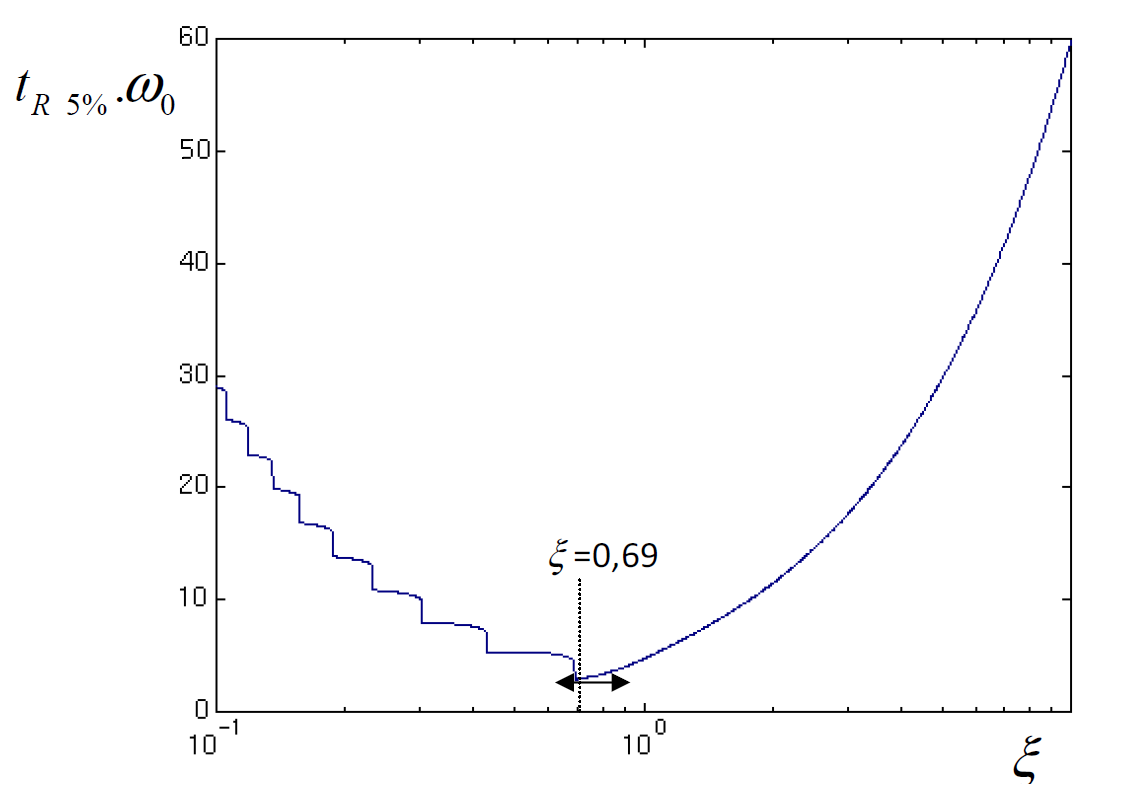
\includegraphics[width=0.7\linewidth]{img/maxpid4.png}
 \caption{Temps de réponse à 5\%}
 \label{maxpid4}
\end{figure}
\newpage

L'inertie proposée précédemment correspondait au Maxpid avec les masses. En enlevant ces masses l'inertie équivalente devient $J=0,0005kg.m^2$.

\paragraph{Question 9 :} Appliquer les modifications revoir les valeurs de $K$, $\xi$ et $\omega_0$. Quel sera l'impact sur le système ?

\paragraph{Question 10 :} Tracer l'allure de la réponse. Déterminer les nouvelles caractéristiques de cette réponse.

Pour éviter tout mouvement brusque du Maxpid, il a été décidé de le piloter par une loi de tension en trapèze, ce qui revient dans un premier temps à alimenter le moteur avec la loi $u(t)=e_0.t$, avec $e_0=\pi$. Appliquer cette loi sur le système avec les 3 masses, c'est à dire, avec $J=0,01kg.m^2$.

\paragraph{Question 11 :} Déterminer la réponse temporelle $\omega(t)$ dans ce cas, tracer cette réponse et la commenter. Pour cela, déterminer les deux pôles de la fonction de transfert et simplifier son écriture grâce à une approximation.

\newpage

\section{Diravi}

\begin{figure}[!h]
\begin{minipage}{0.45\linewidth}
Le but de cette étude de MODELISER le comportement d'un actionneur et de son pré-actionneur à l'aide d'un
modèle de connaissance.

L'actionneur étudié est un vérin d'assistance hydraulique.

C'est un constituant du système de direction assistée DIRAVI équipant les véhicules Citroën XM.
\end{minipage}
\hfill
\begin{minipage}{0.5\linewidth}
 \centering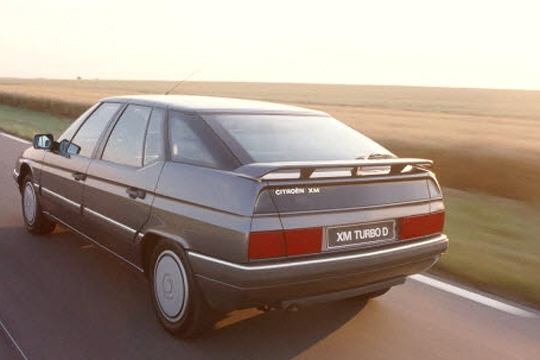
\includegraphics[width=0.7\linewidth]{img/diravi1.jpg}
  \caption{Véhicule équipé de la Diravi}
 \label{diravi1}
\end{minipage}
\end{figure}

Cet actionneur sera caractérisé par sa fonction de transfert et par une étude temporelle par sa réponse indicielle. 
La démarche utilisée met en place un modèle de connaissance.

En plus du classique système mécanique de direction (volant, colonne de direction, pignon, crémaillère?), l'ensemble d'assistance est constitué :
\begin{itemize}
 \item D'un vérin d'assistance, commandant la crémaillère de direction et donc le pivotement des roues,
 \item D'un groupe hydraulique (pompe hydraulique entraînée par un motoréducteur, réservoir d'huile, accumulateur de pression et conjoncteur-disjoncteur) gérant le débit et la pression du fluide,
 \item D'un bloc de commande que l'on peut diviser en deux sous-ensembles,
 \begin{itemize}
 \item Un comparateur qui permet de piloter le système hydraulique de braquage des roues en fonction de la position du volant,
 \item Un système came-poussoir qui exerce un couple de rappel, variable en fonction de la position du volant.
\end{itemize}
 \item D'un régulateur centrifuge, qui permet de faire varier le couple de rappel au neutre du volant en fonction de la vitesse du véhicule.
\end{itemize}

\begin{figure}[!h]
 \centering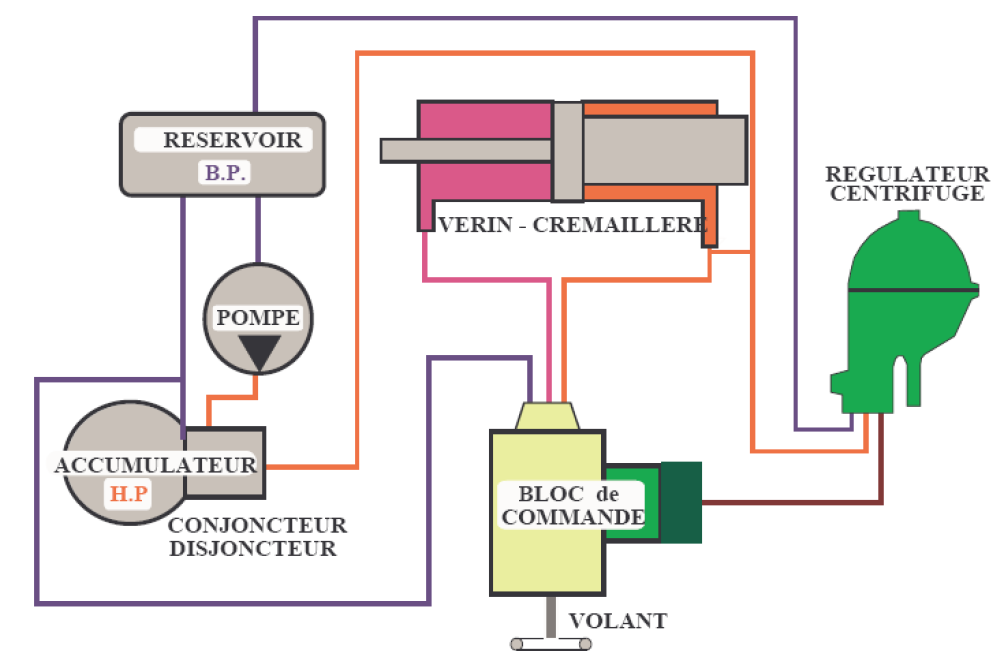
\includegraphics[width=0.7\linewidth]{img/diravi2.png}
 \caption{Composants de la diravi}
 \label{diravi2}
\end{figure}

Une description simplifiée du circuit hydraulique est donnée ci-dessous.

\begin{figure}[!h]
 \centering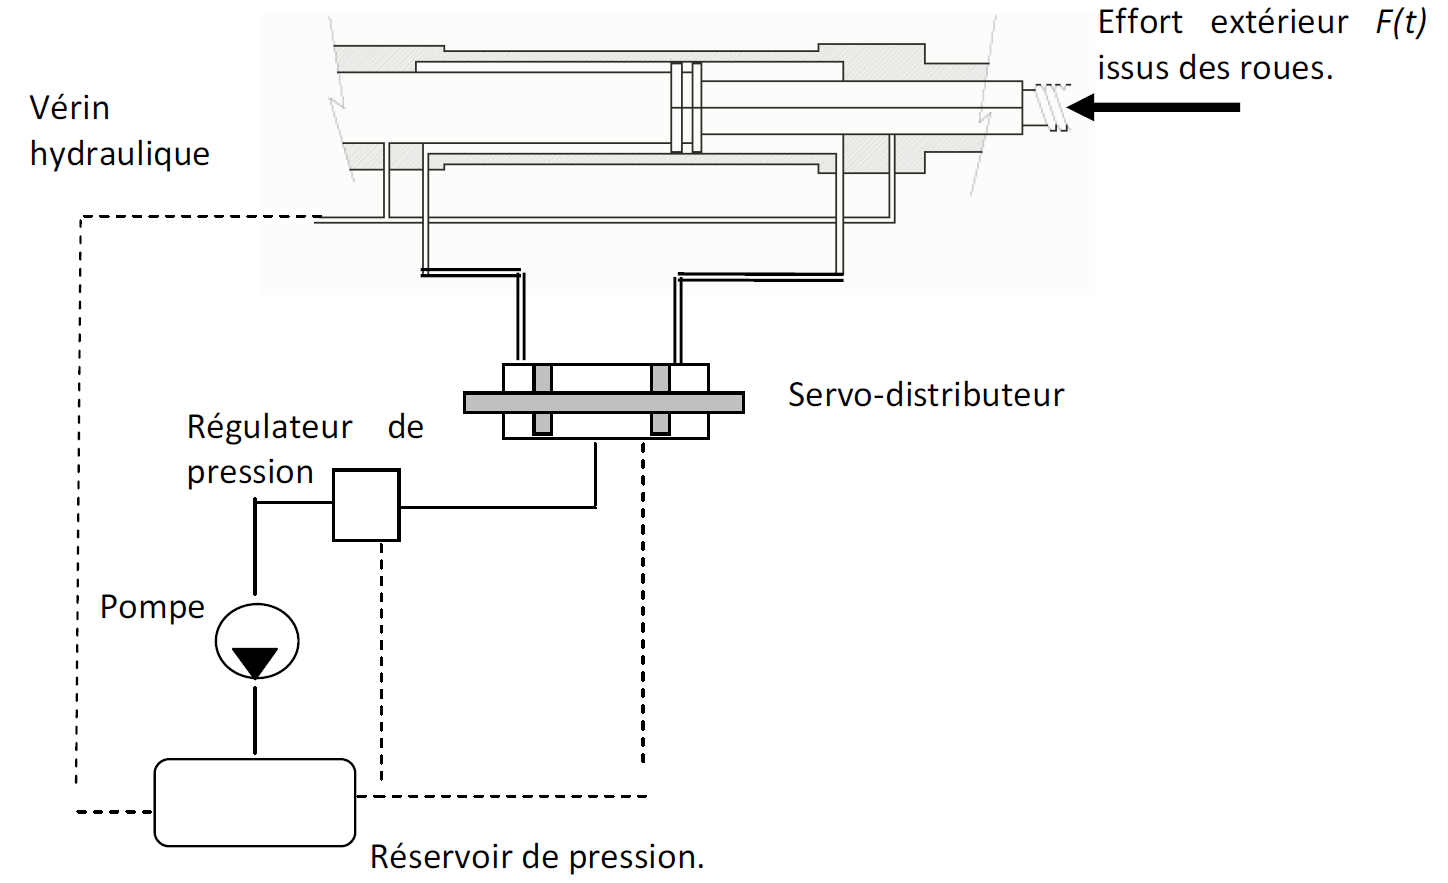
\includegraphics[width=0.7\linewidth]{img/diravi3.png}
 \caption{Circuit hydraulique}
 \label{diravi3}
\end{figure}

\subsection{1ère étude : Cas d'un système déplaçant une masse nulle à l'aide d'un fluide incompressible et sans fuite}

\begin{figure}[!h]
 \centering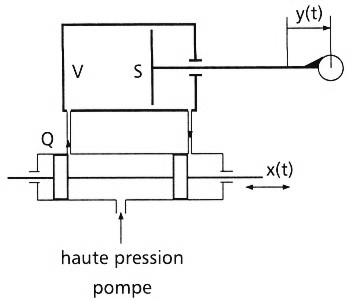
\includegraphics[width=0.4\linewidth]{img/diravi4.png}
 \caption{Servo-distributeur}
 \label{diravi4}
\end{figure}

Comportement du servo-distributeur : Le débit volumique $Q$ est proportionnel au déplacement du tiroir du distributeur $x$ : $Q(t)=k.x(t)$ (1).

Comportement du vérin : Le débit volumique Q est lié à la vitesse de déplacement de la tige paramétrée par le
déplacement y et à la section du vérin : $Q(t)=S.\dot{y}(t)$ (2).

Le signal reçu en entrée $x$ est un échelon unité $u$. La réponse y obtenue en sortie est appelée réponse indicielle du système. Pour $t<0$, $y(t)=0$.

\paragraph{Question 1:} Représentez ce système à l'aide d'une chaîne fonctionnelle.

\paragraph{Question 2:} Déterminez l'équation différentielle qui lie $x(t)$ et $y(t)$.

\paragraph{Question 3:} Déterminez la fonction de transfert $H_1(p)=\frac{Y(p)}{X(p)}$. Mettre cette fonction de transfert sous la forme canonique : $H_1(p)=\frac{K^*}{p}$. Déterminer $K^*$.

\paragraph{Question 4:} Donnez la valeur de $Y(p)$ la transformée de Laplace de la réponse indicielle.

\paragraph{Question 5:} En déduire sa réponse temporelle. 

\subsection{2ème étude : Cas d'un système déplaçant une masse à l'aide d'un fluide incompressible avec une fuite}

Le comportement du distributeur est inchangé.
On note $\Delta_p$ la différence de pression entre les deux chambres du vérin.

\begin{figure}[!h]
 \centering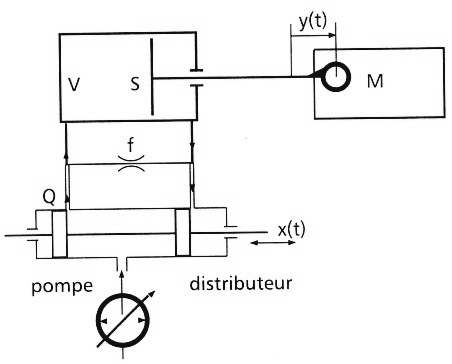
\includegraphics[width=0.4\linewidth]{img/diravi5.png}
 \caption{Servo-distributeur}
 \label{diravi5}
\end{figure}

Comportement du vérin : L'équation cinématique en débit (2) reste valable. Il faut ajouter le dédit de perte $Q_p$ par fuite entre les deux chambres : $Q_p=f.\Delta_p(t)$ où $f$ est un coefficient constant.

L'intensité de la force appliquée $F$ à la masse $M$ par le vérin est proportionnelle de l'aire de la section $S$ du vérin à la différence de pression entre les deux chambres $\Delta_p$ : $F(t)=S.\Delta_p(t)$ (4).

Conservation du débit dans le circuit hydraulique : Il faut ajouter à l'équation (2) le débit de perte : $Q(t)=S.\dot{y}(t)+Q_p(t)$ (2').

Comportement de la masse : Il est donné par le principe fondamental de la dynamique appliqué à la masse $M$ en
mouvement dans un référentiel Galiléen. L'équation de résultante projetée sur la direction horizontale donne :
$F(t)=M.\ddot{y}(t)$ (5).

\paragraph{Question 6:} Transformez les équations différentielles données dans le domaine de Laplace en utilisant
des conditions initiales nulles.

\paragraph{Question 7:} En déduire la fonction de transfert du système : $H_2(p)=\frac{Y(p)}{X(p)}$.

\paragraph{Question 8:} Mettre cette fonction de transfert sous forme canonique. Indiquez la classe, l'ordre, le
gain et les caractéristiques du système.

%\paragraph{Question 9:} Déterminez la réponse temporelle indicielle de ce système.
%
%\subsection{3ème étude : Cas d'un système déplaçant une masse à l'aide d'un fluide compressible avec
%une fuite (système du second ordre)}
%
%La modélisation précédente reste valable. Il faut modifier l'équation des débits pour ajouter
%le débit équivalent tenant compte de la compressibilité du fluide $Q_c$ : $Q(t)=S.\dot{y}(t)+Q_p(t)+Q_c(t)$ (2'').
%
%Comportement du fluide : Le comportement compressible du fluide est décrit par sa diminution de volume $Q_c$ due à sa compressibilité : $Q_c(t)=\left(\frac{V}{2}.\beta\right)\frac{d(\Delta_p(t))}{dt}$ (6).
%
%Le terme $\left(\frac{V}{2}.\beta\right)$ est considéré comme une constante du fluide.
%
%\paragraph{Question 10:} Transformez les équations différentielles données dans le domaine de Laplace en utilisant
%des conditions initiales nulles.
%
%\paragraph{Question 11:} En déduire la fonction de transfert du système :$H_2(p)=\frac{Y(p)}{X(p)}$.
%
%
%\paragraph{Question 12:} Mettre cette fonction de transfert sous forme canonique. Indiquez la classe, l'ordre, le
%gain et les caractéristiques du système.
%
%\paragraph{Question 13:}Déterminez la réponse indicielle de ce système.

\newpage

\section{Presse cisaille}

La société COPEX, installée à Lanester (56 Morbihan) est spécialisée dans les machines et leurs applications à l'environnement. Elle conçoit et fabrique, en particulier du matériel permettant de compacter des déchets de différentes natures, afin d'éventuellement les retraiter ou de les stocker.

L'étude proposée porte sur une Presse-Cisaille type CVB 1 000 T (Cisaille Verticale à Bac de 1 000 tonnes) destinée à traiter de la ferraille de toute sorte. En fonction des matériaux récupérés, elle permet le compactage sous forme de paquet ou le cisaillage afin de diminuer les volumes lors du transport avant retraitement ou stockage final.

Le déplacement en translation du tiroir est assuré par deux vérins hydrauliques $V_1$ et $V_2$ nécessitant un palonnier pour éviter l'arc-boutement lors de son déplacement.

Cette étude porte sur une nouvelle solution remplaçant le palonnier par un asservissement en position des deux vérins.

Les deux vérins hydrauliques sont montés en portique en deux points d'ancrage (en parallèle) sur le tiroir. Chaque vérin du type \og mesure en position intégrée \fg (détecteur inductif intégré dans la tige du vérin, résolution $\pm 0,1$ mm) est piloté par un servo-distributeur. Les commandes des deux vérins sont synchronisées pour limiter l'arc-boutement du tiroir (efforts dissymétriques dus à la ferraille à compacter).

On isole l'un des vérins.

Le comportement du vérin peut alors être modélisé à partir du modèle de structure ci-dessous et du paramétrage qui lui est associé.

\begin{figure}[!h]
 \centering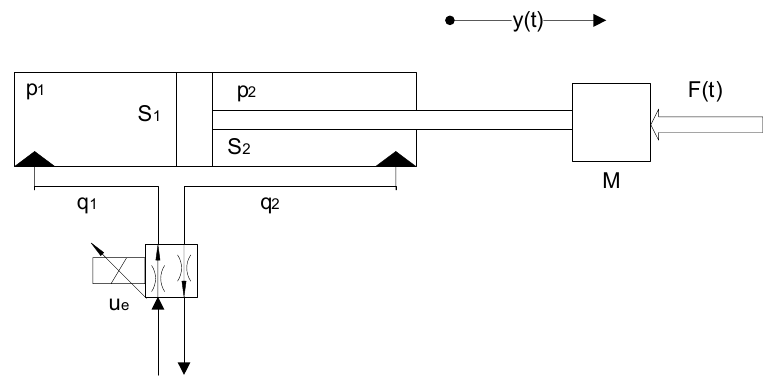
\includegraphics[width=0.6\linewidth]{img/fig3.png}
\end{figure}

On donne :
\begin{itemize}
 \item $M=10^4kg$ : masse de l'équipage mobile ;
 \item $f=3.10^6N/m/s$ : la résistance due aux frottements visqueux ;
 \item $K=2,5.10^7N/m$ : la raideur hydraulique du vérin ;
 \item $S_1=5.10^{-2}m^2$ : la surface du piston de la chambre d'admission.
\end{itemize}

L'ensemble appelé \og équipage mobile \fg est formé par :
\begin{itemize}
 \item le tiroir,
 \item l'effort variable dû à la ferraille, noté F(t),
 \item la tige du piston du vérin.
\end{itemize}

Sa position notée y(t) est fonction du débit d'huile, noté $q_1(t)$, à l'entrée de la chambre d'admission du vérin.

On se place dans l'hypothèse de petit déplacement autour d'un point de fonctionnement (position particulière d'équilibre). Le système peut donc être considéré comme linéaire, continu et invariant.

\paragraph{Modélisation de l'équipage mobile}

Après calcul :
\begin{itemize}
 \item L'équation temporelle donnant le déplacement $y_1(t)$ en fonction du débit $q_1(t)$ pour un effort $F(t)$ nul est telle que : 
 $M.\frac{d^2y_1(t)}{dt^2}=K.\int_{0}^{t} \frac{q_1(\tau)}{S_1}d\tau-K.y_1(t)-f.\frac{dy_1(t)}{dt}$
 \item L'équation temporelle donnant le déplacement $y_2(t)$ en fonction de l'effort $F(t)$ pour un débit $q_1(t)$ nul est telle que :
 $M.\frac{d^2y_2(t)}{dt^2}=-K.y_2(t)-f.\frac{dy_2(t)}{dt}+F(t)$
\end{itemize}

\paragraph{Question 1 :} En supposant que les conditions initiales sont nulles, donner dans le domaine de Laplace et sous forme canonique les fonctions de transfert:

\begin{itemize}
 \item $H_1(p)=\frac{Y_1(p)}{Q_1(p)}$ liant le déplacement $y_1(t)$ au débit $q_1(t)$ pour un effort $F(t)$ nul,
 \item $H_2(p)=\frac{Y_2(p)}{F(p)}$ liant le déplacement $y_2(t)$ à l'effort $F(t)$ pour un débit $q_1(t)$ nul.
\end{itemize}
  
\paragraph{Question 2 :} En appliquant le principe de superposition, donner l'équation, dans le domaine de Laplace, liant le déplacement $Y(p)$ au débit $Q_1(p)$ et à l'effort $F(p)$.

\newpage

\section{Moteur à courant continu en charge}

Le fait e connecter une charge (de type couple résistant) à un moteur à courant continue revient à modifier son équation mécanique comme suit (ajouter $C_r(t)$):

\begin{minipage}{0.40\linewidth}
 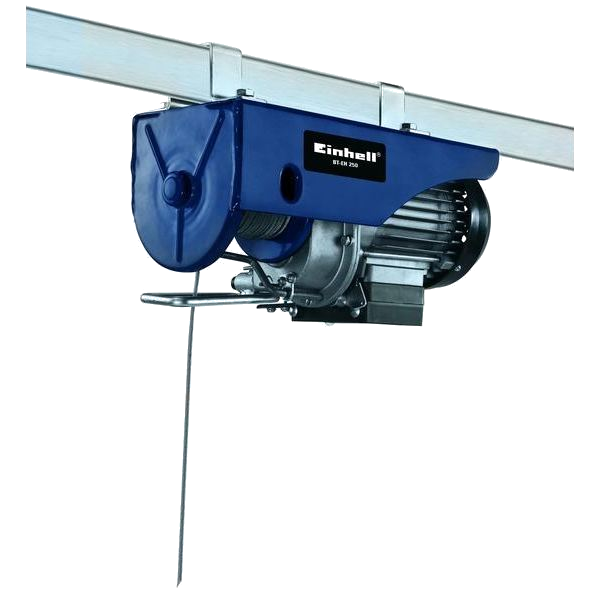
\includegraphics[width=0.8\linewidth]{img/treuil}
\end{minipage}\hfill
\begin{minipage}{0.50\linewidth}
\begin{eqnarray}
u_m(t)=R.i(t)+L.\frac{di(t)}{dt}+e(t) \\
e(t)=K_e.\omega(t) \\ 
C_m(t)=K_t.i(t) \\
J.\dfrac{d\omega (t)}{dt}=C_m(t)-C_r(t)-f.\omega(t)
\end{eqnarray}
\end{minipage}

On donne les valeurs numériques suivantes:\\
\begin{minipage}{0.45\linewidth}
\begin{itemize}
 \item $R=2,5\Omega$,
 \item $L=7,5.10^{-3}H$,
 \item $Ke=11,5.10^{-3}.\frac{60}{2.\pi}=0,11 V.rad^{-1}.s$
\end{itemize}
\end{minipage}\hfill
\begin{minipage}{0.45\linewidth}
\begin{itemize}
 \item $Kc=0,11N.m.A^{-1}$,
 \item $J=5.10^{-5}kg.m^2$,
 \item $f=0,01N.m.rad^{-1}.s$
\end{itemize}
\end{minipage}

\paragraph{Question 1:} Donner les équations temporelles de (1) à (4) dans le domaine de Laplace

\paragraph{Question 2:} Trouver la fonction de transfert $H_1(p)$ quand $C_r(p)=0$.

\paragraph{Question 3:} Trouver la fonction de transfert $H_2(p)$ quand $U_m(p)=0$.

\paragraph{Question 4 :} Mettre ces fonctions de transfert sous forme canonique et identifiez leur classes, ordres et leurs constantes caractéristiques.

\paragraph{Question 5 :} Faire l'application numérique.

\paragraph{Question 6:} Tracer la réponse temporelle $s(t)$ pour une entrée en échelon $u_m(t)=20V$ avec un effort résistant nul $c_r(t)=0N.m$.

\section{Transformée de Laplace de fonctions usuelles}

\begin{center}
\begin{tabular}{|c|c||c|c|}
\hline
Temporel $f(t)$ & Laplace $F(p)$ & 
Temporel $f(t)$ & Laplace $F(p)$ \\
\hline
\hline
 &&& \\
Dirac $\delta(t)$ &
$F(p)=1$ &
Échelon $ u(t)=k $&
$ U(p) = \frac{k}{p}$
\\
&&& \\
\hline
&&& \\
$f(t) = t^n\cdot u(t)$ &
$F(p)=\frac{n!}{p^{n+1}} $ &
$\forall t\in ]0,t_1 [ \quad f(t)= A$ & 
$F(p) =A \cdot \frac{1-e^{-pt_1}}{p} $\\
&&& \\
\hline
&&& \\
$f(t) = \sin \left( \omega_0 t\right) \cdot u(t)$ &
$F(p) = \frac{\omega_0}{p^2+\omega_0^2} $ &
$f(t) = \cos \left( \omega_0 t\right) \cdot u(t)$ & 
$F(p) = \frac{p}{p^2+\omega_0^2} $ \\
&&& \\
\hline
&&& \\
$f(t)= e^{-at}\cdot u(t)$ & 
$F(p)= \frac{1}{p+a}$ &
$f(t) = e^{-at}\sin\left( \omega_0 t\right) \cdot u(t)$ &
$f(t)=\frac{\omega_0}{\left( p+a\right)^2 + \omega_0^2}$  \\
&&& \\
\hline
&&& \\
$f(t) = e^{-at}\cos\left( \omega_0 t\right) \cdot u(t)$ &
$f(t)=\frac{p+a}{\left( p+a\right)^2 + \omega_0^2}$  &
$f(t)=t^ne^{-at}u(t)$ & $F(p)=\frac{n!}{\left( p+a\right)^{n+1}}$ \\
&&& \\
\hline
\end{tabular}
\end{center}

\ifdef{\public}{\end{document}}{}

\newpage

\pagestyle{correction}

\section{Correction}

\subsection{Maxpid}

\paragraph{Question 1:}

\begin{itemize}
 \item Résistance: $u_R(t)=R.i(t)$,
 \item Inductance: $U_L(t)=L.\dfrac{di(t)}{dt}$,
 \item Équation différentielle: $u(t)=e(t)+R.i(t)+L.\dfrac{di(t)}{dt}$ (en prenant le signe en fonction de la convention générateur/récepteur).
\end{itemize}

\paragraph{Question 2:}

\begin{enumerate}
 \item $E(t)=K_e.\Omega(p)$,
 \item $C_m(p)=K_t.I(p)$,
 \item $C_m(p)=f.\Omega(p)+J.p.\Omega(p)$,
 \item $U(p)=E(p)+R.I(p)+L.p.I(p)$.
\end{enumerate}

\paragraph{Question 3:}

D'après l'énoncé, l'entrée est $u(t)$ et la sortie $\omega(t)$.

Donc, $H(p)=\dfrac{\Omega(p)}{U(p)}=\dfrac{K_t}{K_e.K_t+(R+L.p).(f+J.p)}$

\paragraph{Question 4:}

La forme canonique est alors: $H(p)=\dfrac{K}{1+\dfrac{2.\xi}{\omega_0}.p+\dfrac{p^2}{\omega_0^2}}$

$H(p)=\dfrac{\dfrac{K_t}{K_e.K_t+R.f}}{1+\dfrac{L.f+R.J}{K_e.K_t+R.f}.p+\dfrac{L.J}{K_e.K_t+R.f}.p^2}$

\begin{itemize}
 \item Classe:0,
 \item Ordre:2,
 \item Gain:$K=\dfrac{K_t}{K_e.K_t+R.f}$.
\end{itemize}

\paragraph{Question 5:}

Donc,

\begin{itemize}
 \item $\omega_0=\sqrt{\dfrac{K_e.K_t+R.f}{L.J}}$,
 \item $\xi=\dfrac{\omega_0}{2}.\dfrac{L.f+R.J}{K_e.K_t+R.f}=\dfrac{1}{2}.\sqrt{\dfrac{K_e.K_t+R.f}{L.J}}.\dfrac{L.f+R.J}{K_e.K_t+R.f}=\dfrac{L.f+R.J}{2.\sqrt{L.J.(K_e.K_t+R.f)}}$,
\end{itemize}

\paragraph{Question 6:}

Donc,

\begin{itemize}
 \item $K_e=\dfrac{1}{182}V.tr^{-1}.min=\dfrac{1}{182}.\dfrac{30}{\pi}=52,5.10^{-3}V.rad^{-1}.s$,
 \item $K_t=52,5.10^{-3}N.m.A^{-1}$,
 \item $L=0,62.10^{-3}H$,
 \item $R=2,07\Omega$,
 \item $J=0,01kg.m^2$,
 \item $f=0,125N.m.rad^{-1}.s^{-1}$.
\end{itemize}

\begin{itemize}
 \item Gain: $K=\dfrac{K_t}{K_e.K_t+R.f}=\dfrac{52,5.10^{-3}}{52,5.10^{-3}.52,5.10^{-3}+2,07.0,125}=0,2rad.s^{-1}.V^{-1}$,
 \item Pulsation propre du système: $\omega_0=\sqrt{\dfrac{K_e.K_t+R.f}{L.J}}=\sqrt{\dfrac{52,5.10^{-3}.52,5.10^{-3}+2,07.0,125}{0,62.10^{-3}.0,01}}=205,4rad.s^{-1}$,
 \item Facteur d'amortissement: $\xi=\dfrac{0,62.10^{-3}.0,125+2,07.0,01}{2.\sqrt{0,62.10^{-3}.0,01.(52,5.10^{-3}.52,5.10^{-3}+2,07.0,125)}}=8,16$
\end{itemize}

Les pôles du systèmes sont donc des réels négatifs.

\paragraph{Question 7:}

J'ai tracé sur la figure suivante:
\begin{itemize}
 \item la courbe réelle du second ordre,
 \item la courbe approchée en considérant l'inductance nulle.
\end{itemize}

Les figures suivantes représentent un zoom faisant apparaitre la tangente à l'origine.
\begin{center}
	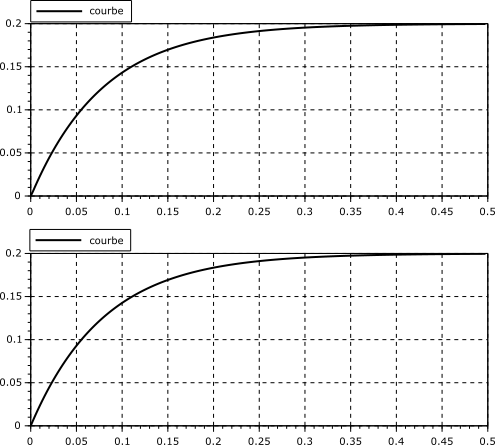
\includegraphics[width=0.7\linewidth]{img/courbe1}
\end{center}

\begin{center}
	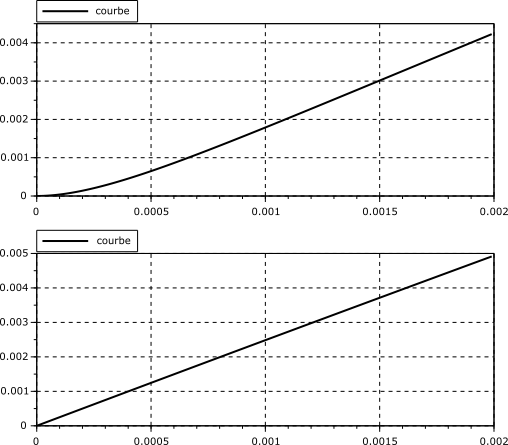
\includegraphics[width=0.7\linewidth]{img/courbe1_2}
\end{center}

La construction de la courbe s'effectue en utilisant la tangente en chaque point.

\begin{center}
	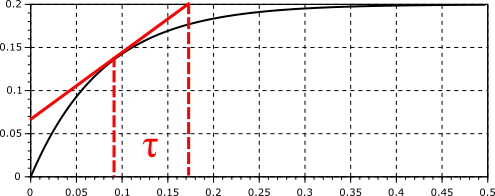
\includegraphics[width=0.7\linewidth]{img/tau}
\end{center}

Et on trouve le temps de réponse avec la construction suivante.

\begin{center}
	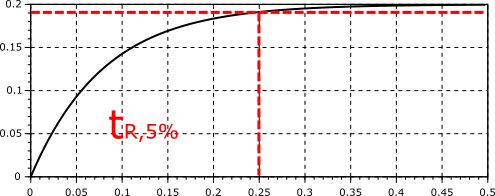
\includegraphics[width=0.7\linewidth]{img/temps_rep}
\end{center}
	
\paragraph{Question 8:}

Le temps de réponse est donc: $t_{R,5\%}.\omega_0=50$, donc $t_{R,5\%}=\dfrac{50}{205,4}=0,25s$.

%\paragraph{Question 9 :} 
%
%Dans ce cas, $K=0,2$, $\xi=0,44$ et $\omega_0=918,46rad.s^-1$. Cela a pour effet de rendre le système instable.
%
%\paragraph{Question 10 :} 
%
%\begin{center}
%	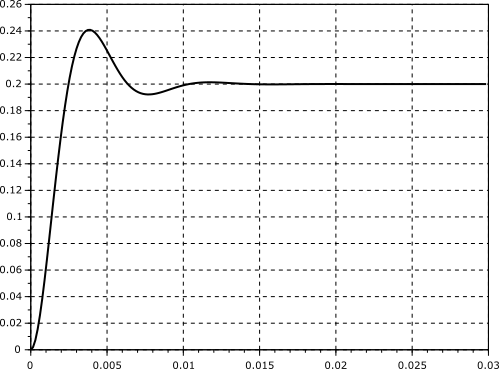
\includegraphics[width=0.7\linewidth]{img/courbe2}
%\end{center}
%
%Cette fois-ci on se rend compte que l'inductance ne peut pas être négligée.
%
%\begin{center}
%	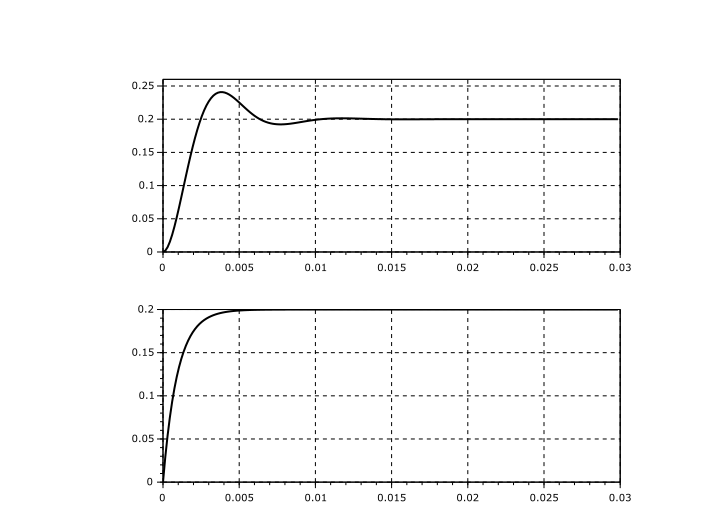
\includegraphics[width=0.7\linewidth]{img/courbe2_2}
%\end{center}
%
%$D\%=100.e^{-\xi.\dfrac{\pi}{\sqrt{1-\xi^2}}}=22\%$, avec une sortie $s(+\infty)=0,2$, cela signifie que le dépassement monte à $0,24$.
%
%$t_{R,5\%}=\dfrac{1}{\xi.\omega_0}.ln(20)=0,0075s$.
%
%$T_p=\dfrac{2.\pi}{\omega_0.\sqrt{1-\xi^2}}$
%
%On retrouve ces valeurs sur le tracé.
%
%\begin{center}
%	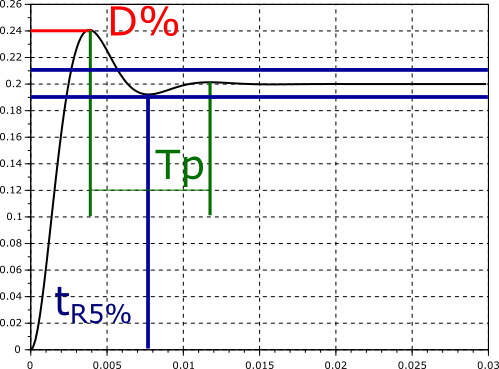
\includegraphics[width=0.7\linewidth]{img/courbe2_3}
%\end{center}
%
%\paragraph{Question 11 :} En reprenant la valeur de $J$ initiale, le système n'oscille plus.
%
%$p_1=-\xi.\omega_0+\omega_0.\sqrt{\xi^2-1}=-12,6rad.s^{-1}$
%
%$p_2=-\xi.\omega_0-\omega_0.\sqrt{\xi^2-1}=-3333rad.s^{-1}$
%
%On constate que, $p_2$ est très grand devant $p_1$.
%
%Ainsi, $(1-\dfrac{p}{p_2})$ peut être considéré équivalent à $1$. C'est toujours le cas dans un système du second ordre lorsque $\xi$ est grand (>4 ou >5).
%
%$H(p)=\dfrac{K}{1-\dfrac{p}{p_1}}=\dfrac{K}{1+\tau.p}$, avec $K=0,2$ et $\tau=0,079$.
%
%$S(p)=\dfrac{K}{1+\tau.p}.\dfrac{\pi}{p^2}$
%
%$s(t)=-0,2.\pi.\tau+0,2.\pi.t+0,2.\pi.\tau.e^{-\dfrac{t}{\tau}}$
%
%$s(t)=0,2.\pi.(t-\tau.(1-.e^{-\dfrac{t}{\tau}})$
%
%Avec $s(+\infty)=0,2.(t-\tau).e_0=0,2.\pi.(t-0,079)$, ce qui explique le décalage des courbes.
%
%\begin{center}
%	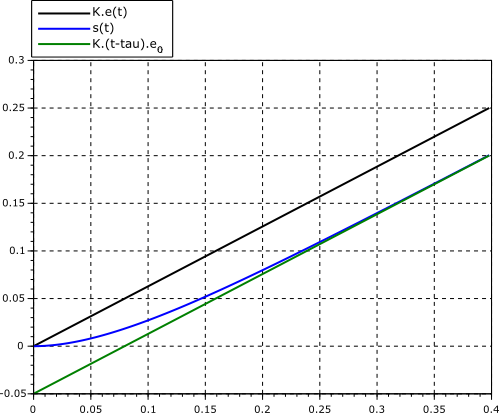
\includegraphics[width=0.7\linewidth]{img/courbe3}
%\end{center}
%
%\begin{center}
%	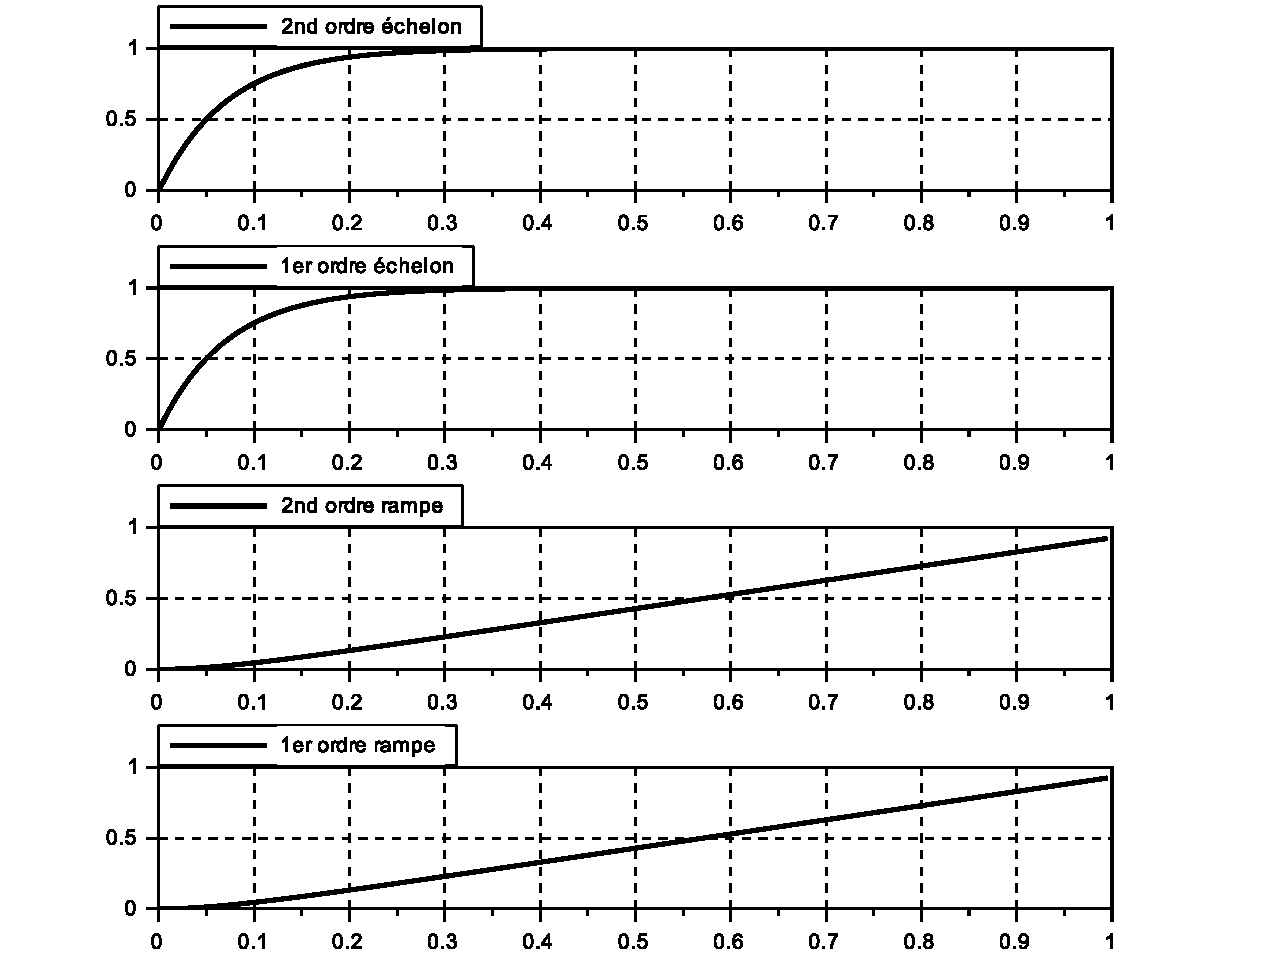
\includegraphics[width=0.7\linewidth]{img/courbe4}
%\end{center}

\subsection{Correction Diravi}

\paragraph{Question 1:}

\begin{itemize}
 \item \textbf{Alimenter:} Réservoir, pompe, accumulateur,
 \item \textbf{Distribuer:} servo-distributeur,
 \item \textbf{Convertir:} vérin,
 \item \textbf{Transmettre:} Rien si on dit que le système agit sur la barre de direction, les biellettes de direction si on dit que le système agit sur les roues,
 \item \textbf{Acquérir:} volant, régulateur centrifuge,
 \item \textbf{Traiter:} bloc de commande,
 \item \textbf{Communiquer:} tuyaux.
\end{itemize}

\paragraph{Question 2:}

$k.x(t)=S.\dot{y}(t)$.

\paragraph{Question 3:}

$H_1(p)=\dfrac{\dfrac{k}{S}}{p}$, donc $K^*=\dfrac{k}{S}$.

\paragraph{Question 4:}

$Y(p)=\dfrac{K^*}{p^2}$

\paragraph{Question 5:}

$y(t)=K^*.t$

\paragraph{Question 6:}

\begin{itemize}
 \item $Q(p)=k.X(p)$,
 \item $Q_p(p)=f.\Delta_p(p)$,
 \item $F(p)=S.\Delta_p(p)$,
 \item $Q(p)=S.p.Y(p)+Q_p(p)$,
 \item $F(p)=M.p^2.Y(p)$.
\end{itemize}

\paragraph{Question 7:}

$k.X(p)=S.p.Y(p)+f.\Delta_p(p)$

$k.X(p)=S.p.Y(p)+f.\dfrac{M.p^2.Y(p)}{S}$

$H_2(p)=\dfrac{k}{S.p+\dfrac{f.M.p^2}{S}}$

\paragraph{Question 8:}

$H_2(p)=\dfrac{\dfrac{k}{S}}{p.\left(1+\dfrac{f.M.p}{S^2}\right)}$

\begin{itemize}
 \item Classe: 1,
 \item Ordre: 2,
 \item Gain: $\dfrac{k}{S}$,
 \item Constante de temps: $\tau=\dfrac{f.M}{S^2}$.
\end{itemize}

\paragraph{Question 9:}

$Y(p)=\dfrac{\dfrac{k}{S}}{p^2.\left(1+\dfrac{f.M.p}{S^2}\right)}$

$Y(p)=\dfrac{A.p+B}{p^2}+\dfrac{C}{1+\dfrac{f.M.p}{S^2}}=\dfrac{\left(C+A.\dfrac{f.M}{S^2}\right).p^2+\left(A+\dfrac{f.M.B}{S^2}\right).p+B}{p^2.\left(1+\dfrac{f.M.p}{S^2}\right)}$

\begin{minipage}{0.49\linewidth}
\begin{itemize}
 \item $C+A.\dfrac{f.M}{S^2}=0$,
 \item $A+\dfrac{f.M.B}{S^2}=0$,
 \item $B=\dfrac{k}{S}$.
\end{itemize}
\end{minipage}\hfill
\begin{minipage}{0.49\linewidth}
\begin{itemize}
 \item $A=-\dfrac{f.M.k}{S^3}$,
 \item $B=\dfrac{k}{S}$,
 \item $C=\dfrac{f^2.M^2.k}{S^5}$.
\end{itemize}
\end{minipage}

$Y(p)=\dfrac{A.p+B}{p^2}+\dfrac{C}{1+\dfrac{f.M.p}{S^2}}$

$y(t)=A+B.t+\dfrac{S^2.C}{f.M}.e^{\dfrac{-S^2.t}{f.M}}$

\paragraph{Question 10:}

\begin{itemize}
 \item $Q(p)=k.X(p)$,
 \item $Q_p(p)=f.\Delta_p(p)$,
 \item $F(p)=S.\Delta_p(p)$,
 \item $Q(p)=S.p.Y(p)+Q_p(p)+Q_c(p)$,
 \item $Q_c(p)=\left(\dfrac{V}{2}.\beta\right).p.\Delta_p(p)$,
 \item $F(p)=M.p^2.Y(p)$.
\end{itemize}

\paragraph{Question 11:}

$k.X(p)=S.p.Y(p)+f.\Delta_p(p)+\left(\dfrac{V}{2}.\beta\right).p.\Delta_p(p)$

$k.X(p)=S.p.Y(p)+\left(f+\left(\dfrac{V}{2}.\beta\right).p\right).\dfrac{M.p^2.Y(p)}{S}$

$H_2(p)=\dfrac{k}{S.p+\dfrac{\left(f+\left(\dfrac{V}{2}.\beta\right).p\right).M.p^2}{S}}$

\paragraph{Question 12:}

$H_2(p)=\dfrac{k}{S.p+\dfrac{\left(f+\left(\dfrac{V}{2}.\beta\right).p\right).M.p^2}{S}}$

\subsection{Presse cisaille}

\paragraph{Question 1:}

En supposant les conditions initiales nulles :

$M.p^2.Y_1(p)=\dfrac{K.Q_1(p)}{S_1.p}-K.Y_1(p)-f.p.Y_1(p)$ d'où on en déduit: $H_1(p)=\dfrac{1/S_1}{p.\left(\dfrac{M}{K}.p^2+\dfrac{f}{K}.p+1\right)}$.

$M.p^2.Y_2(p)=-K.Y_2(p)-f.p.Y_2(p)+F(p)$ d'où on en déduit: $H_2(p)=\dfrac{1/K}{\dfrac{M}{K}.p^2+\dfrac{f}{K}.p+1}$.

\paragraph{Question 2:}

$Y(p)=Y_1(p)+Y_2(p)=H_1(p)\times Q_1(p)+H_2(p)\times F(p)$

$Y(p)=\dfrac{1/S_1}{p.\left(\dfrac{M}{K}.p^2+\dfrac{f}{M}.p+1\right)}.Q_1(p)+
\dfrac{1/K}{\dfrac{M}{K}.p^2+\dfrac{f}{M}.p+1}.F(p)$

\subsection{Moteur à courant continu en charge}

\paragraph{Question 1:} 

\begin{eqnarray}
U_m(p)=R.I_m(p)+L.p.I(p)+E(p) \\
E(p)=Ke.\Omega(p) \\
C_m(p)=Kc.I(p) \\
J.p.\Omega(p)=C_m(p)-C_r(p)+f.\Omega(p)
\end{eqnarray}

\paragraph{Question 2:} $H_1(p)=\frac{{\Omega}(p)}{{U}_{m}(p)}=\frac{K_c}{K_e.K_c+R.f} \cdot \frac{1}{1+\frac{R.J+L.f}{K_e.K_c+R.f}.p+\frac{L.J}{K_e.K_c+R.f}.p^2}$

\paragraph{Question 3:} $H_2(p)=\frac{{\Omega}(p)}{C_r(p)}=\frac{-(L.s+R)}{K_e.K_c+R.f} \cdot \frac{1}{1+\frac{R.J+L.f}{K_e.K_c+R.f}p+\frac{L.J}{K_e.K_c+R.f}.p^2}$

\paragraph{Questions 4 et 5:} 

\begin{itemize}
	\item Gain:  $G=\frac{K_c}{K_e.K_c+R.f}=2,97$
	\item Amortissement: $\xi=\frac{R.J+L.f}{2.\sqrt{(K_e.K_c+R.f).L.J}}=\frac{2,5.5.10^{-5}+7,5.10^{-3}.0,01}{2.\sqrt{(0,11.0,11+3,5.10^{-2}).7,5.10^{-3}.5.10^{-5}}}=\frac{10}{\sqrt{3,621.37,5}}\simeq\frac{10}{\sqrt{36.36*10^{-1}}}\simeq\frac{31,6}{36}\simeq\frac{31,6}{36}\simeq0,87$
	\item Pulsation propre: $\omega_0=\sqrt{\frac{K_e.K_c+R.f}{L.J}}=\sqrt{\frac{0,11.0,11+2,5.0,01}{7,5.10^{-3}.5.10^{-5}}}=
\sqrt{\frac{37,1*10^{-3}}{37,5*10^{-8}}}\simeq\sqrt{10}*100\simeq 316rad.s^{-1}$
\end{itemize}

\paragraph{Question 6:} 

\begin{center}
 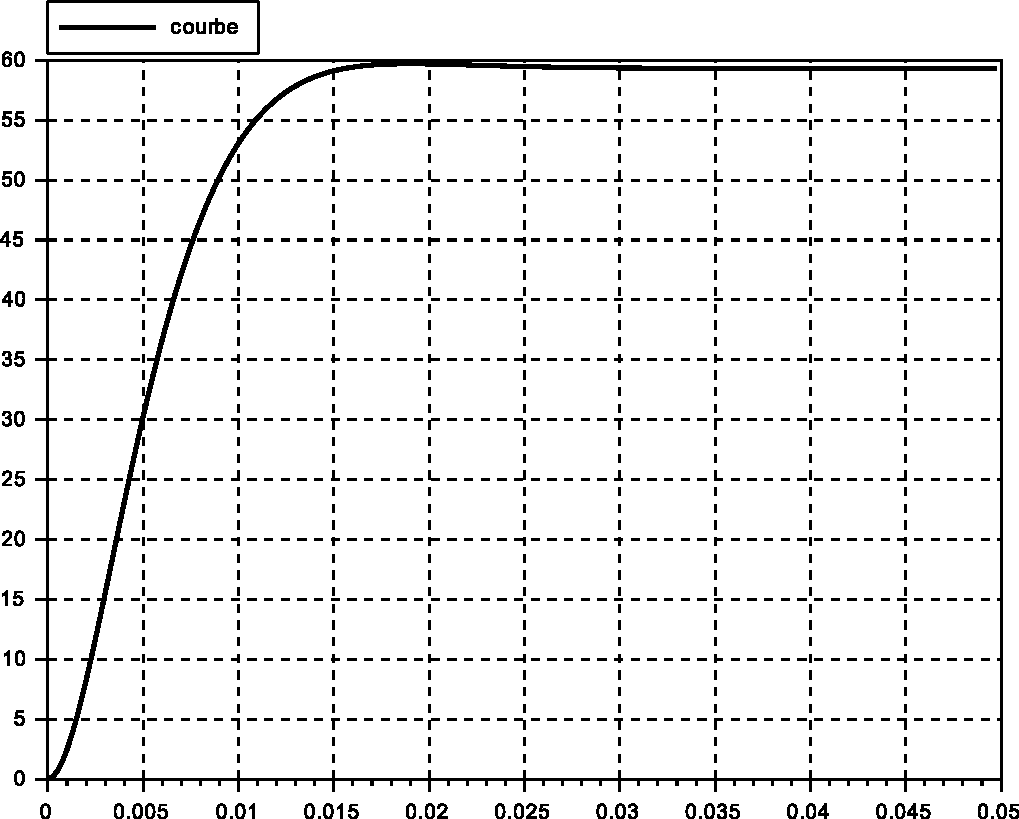
\includegraphics[width=0.8\linewidth]{img/Figure_moteur_charge}
\end{center}

\end{document}


\section{Asservissement en température d'un four (1er ordre) de type proportionnel dérivé}

On considère l'asservissement de température du système constitué d'un four et d'un capteur de température associé.

Avec : 
\begin{itemize}
 \item $\theta_c(t)$ : tension de consigne [V]. Elle représente la température de consigne désirée pour le four (par rapport à la température ambiante),
 \item $\theta(t)$ : tension de mesure [V]. C'est la tension image de la température intérieure du four délivrée par le capteur (exprimée par rapport à la température ambiante),
 \item $p(t)$ : puissance électrique délivrée au four [W]. 
 \item $\varepsilon(t)$ : erreur entre la consigne et la mesure [V].
\end{itemize}

La loi de commande est telle que : 
$p(t)=K_c.[\varepsilon(t)+\tau_d.\frac{\mathrm{d}\varepsilon(t)}{\mathrm{d}t}]$ avec $K_c$ gain statique et $\tau_d$ constante de dérivation.

Et les équations de fonctionnement du système conduisent à :
$\theta(t)+\tau.\frac{\mathrm{d}\theta(t)}{\mathrm{d}t}=K.p(t)$
avec $K$ gain statique du système et $\tau$ constante de temps du système.

\paragraph{Question 1:} Exprimer l'équation différentielle liant $\theta_c(t)$ et $\theta(t)$.

Les conditions initiales sont nulles.

\paragraph{Question 2:} Donner la transformée de Laplace de l'équation différentielle trouvée à la question 1.

\paragraph{Question 3:} Mettre cette équation sous la forme $\Theta(p)=G(p).\Theta_c(t)$.

On considère une consigne échelon $\theta_c(t)=\theta_0.u(t)$ avec $\theta_0$ constante réelle. 

\paragraph{Question 4:} Quelles sont alors les valeurs initiales et finales de la fonction $\theta(t)$ ?

\paragraph{Question 5:} Exprimer $P(p)$ en fonction de $\Theta_c(p)$.

\paragraph{Question 6:} En déduire les valeurs initiale et finale de la commande $p(t)$ pour $\theta_c(t)=\theta_0.u(t)$.

On considère $\tau_d=\tau=60\ s$, $K=0,01\ V/W$ et $\theta_0=7\ V$.

\paragraph{Question 7:} Tracer sur le même graphe : $\theta_c(t)$, $\theta(t)$ et $p(t)$ pour $K_c=100$.
